\documentclass[12pt,a4paper]{report}

\usepackage[utf8]{inputenc}
\usepackage[T1]{fontenc}
\usepackage[polish]{babel}
\usepackage{amsmath}
\usepackage{amsfonts}
\usepackage{amssymb}
\usepackage{graphicx}
\usepackage{booktabs}
\usepackage{subcaption}
\usepackage{hyperref}
\usepackage{listings}
\usepackage{geometry}

\geometry{margin=2.5cm}

\title{Uczenie silnika szachowego na partiach o rosnącym Elo}
\author{Adam Zieliński}
\date{\today}

\begin{document}

\begin{titlepage}
    \centering
    \vspace*{1cm}
    {\Large Uniwersytet Mikołaja Kopernika w Toruniu\\ Wydział Matematyki i Informatyki \par}
    \vspace{3cm}
    {\Huge \textbf{Uczenie silnika szachowego na partiach o rosnącym Elo} \par}
    \vspace{2cm}
    {\Large Praca magisterska \par}
    \vspace{2cm}
    {\Large Autor: Adam Zieliński \par}
    {\Large Promotor: dr hab. Łukasz Mikulski, prof. UMK \par}
    \vfill
    {\Large Toruń, 2026 \par}
\end{titlepage}

\tableofcontents

\chapter*{Streszczenie}

Niniejsza praca bada wpływ uczenia programowego (\textit{curriculum learning})~\cite{bengio2009curriculum} na proces trenowania funkcji ewaluacji pozycji w silnikach szachowych opartych na architekturze NNUE (\textit{Efficiently Updatable Neural Network})~\cite{nasu2018nnue}. Głównym celem badawczym było zweryfikowanie hipotezy, czy sekwencyjne douczanie modelu na partiach pochodzących z coraz wyższych przedziałów rankingowych (Elo) pozytywnie wpłynie na proces optymalizacji, dynamikę funkcji straty oraz końcową siłę gry w porównaniu do podejścia klasycznego (trening na zbiorze o wymieszanym rozkładzie rankingowym, bądź czerpanie jedynie z rozgrywek na poziomie arcymistrzowskim).

Podstawowym celem projektu było stworzenie wirtualnego asystenta do gry w szachy, który grając z użytkownikiem dynamicznie dopasowywał się do jego poziomu, tak aby ciągle odczuwał zaangażowanie bez emocji takich jak frustracja gdy przeciwnik wykorzystuje zbyt skomplikowane dla gracza taktyki, bądź znudzenie gdy taktyki są banalne. We wstępnych pracach nad projektem asystent został zamieniony na wyżej opisany eksperyment aby zweryfikować potencjalną metodę implementacji omawianego asystenta. 

Pierwsze próby stworzenia własnego NNUE odbywały się na architekturze oferowanej przez Leela Chess Zero (\textit{LC0})~\cite{lc0}, jednak ze względu na problemy związane z dokumentacją oraz oferowanymi rozwiązaniami dla kart graficznych marki AMD, na której miał być obliczany eksperyment, postanowiłem zrezygnować z LC0 na rzecz Stockfish~\cite{stockfish}, który okazało się ma rozbudowane repozytorium z narzędziami do trenowania i ogólnej pracy z NNUE nnue-pytorch~\cite{nnuepytorch}. Pracowałem na wersji z 28 marca 2026r, z cechami \textit{HalfKAv2\_hm\string^}, o których opowiem później.

Zbiorami danych wejściowych była oficjalna baza danych serwisu Lichess z marca 2026 roku (ponad 90 milionów pojedynków). Przy użyciu potoku przetwarzania używając własnego skryptu oraz narzędzia \texttt{pgn-extract} surowe partie PGN przefiltrowałem pod kątem minimalnej długości wariantów (\texttt{--minply 40}), poprawności zakończeń (\texttt{--nobadresults}) oraz wyeliminowania asymetrii rankingowej. Przefiltrowane dane podzieliłem na rozłączne koszyki Elo (po 2 miliony gier w każdym), patrząc na średnią arytmetyczną zapisanych rang obydwu graczy. Następnie przetransformowałem je do binarnego formatu \texttt{.binpack} którego wymaga skrypt treningowy.

W celach weryfikacyjnych przeprowadziłem eksperymenty porównawcze obejmujące trzy próby:
\begin{enumerate}
    \item \textbf{Badawczą (curriculum learning):} uczenie realizowane kolejno od najniższych do najwyższych koszyków Elo.
    \item \textbf{Kontrolną:} uczenie na losowo wymieszanym zbiorze danych z pełnego zakresu Elo.
    \item \textbf{Odwróconą:} uczenie rozpoczynane od partii o wysokim Elo, a kończone na partiach graczy początkujących.
\end{enumerate}

W ramach pracy napisałem od podstaw autorski silnik szachowy w języku Python (PyNNUE), który samodzielnie wczytuje zoptymalizowane wagi z plików w formacie \texttt{.nnue} obsługując dekompresję LEB128. Silnik opiera się na algorytmie Alpha-Beta~\cite{russell2010ai}, co uniezależniło platformę testową od obszernego i skomplikowanego kodu C++ Stockfisha. Głównym wnioskiem naukowym płynącym z badań jest to, że zaobserwowane wstrząsy oraz nagłe skoki funkcji straty (Loss Spikes) podczas przełączania koszyków Elo wynikają wyłącznie z drastycznej zmiany dystrybucji samych danych (zjawisko \textit{Co-Domain Shift})~\cite{quinonero2009dataset}. Hipoteza sugerująca, że partie silniejszych szachistów są trudniejsze do zoptymalizowania dla sieci, została przeze mnie obalona. Przeprowadzona próba odwrócona (uczenie od partii z bardzo wysokim Elo w dół) wykazała symetrię problemu, generując bardzo podobne wstrząsy podczas każdej zmiany koszyka, a różnica w całkowitym odchyleniu standardowym między obiema próbami wyniosła zaledwie 3,9\%.

\section*{Abstract}

This thesis investigates the impact of curriculum learning on the process of training the position evaluation function in chess engines based on the NNUE (\textit{Efficiently Updatable Neural Network}) architecture. The main research objective was to verify the hypothesis of whether sequentially training the model on games from progressively higher rating (Elo) brackets would positively affect the optimization process, loss function dynamics, and final playing strength compared to the classic approach (training on a dataset with a mixed rating distribution, or relying solely on grandmaster-level games).

The primary goal of the project was to create a virtual chess assistant that, while playing with the user, would dynamically adapt to their level. This would ensure the player remains engaged without experiencing frustration from overly complex tactics or boredom from trivial ones. During the preliminary work, the assistant was replaced by the aforementioned experiment to verify a potential implementation method for the assistant.

Initial attempts to create a custom NNUE were based on the architecture provided by Leela Chess Zero (\textit{LC0}). However, due to documentation issues and limited support for AMD graphics cards—on which the experiment was to be computed—I decided to switch from LC0 to Stockfish, which proved to have a comprehensive repository of tools for training and working with NNUE (nnue-pytorch). I worked with the version from March 28, 2026, utilizing the \textit{HalfKAv2\_hm\string^} features, which will be discussed later.

The input data consisted of the official Lichess database from March 2026 (over 90 million games). Using a custom data processing pipeline and the \texttt{pgn-extract} tool, I filtered raw PGN files for a minimum game length (\texttt{--minply 40}), proper game endings (\texttt{--nobadresults}), and the elimination of rating asymmetry. The filtered data was divided into disjoint Elo buckets (2 million games each) based on the arithmetic mean of both players' ratings. Subsequently, these were transformed into the binary \texttt{.binpack} format required by the training script.

For verification purposes, I conducted comparative experiments involving three trials:
\begin{enumerate}
    \item \textbf{Research (curriculum learning):} training performed sequentially from the lowest to the highest Elo buckets.
    \item \textbf{Control:} training on a randomly mixed dataset covering the full Elo range.
    \item \textbf{Reversed:} training starting with high-Elo games and ending with beginner games.
\end{enumerate}

As part of the thesis, I developed a custom chess engine in Python (PyNNUE) from scratch, which independently loads optimized weights from \texttt{.nnue} files and supports LEB128 decompression. The engine relies on the Alpha-Beta algorithm, which decoupled the testing platform from Stockfish's extensive and complex C++ codebase. The main scientific conclusion from the research is that the observed tremors and sudden loss function spikes during Elo bucket transitions are caused exclusively by a drastic change in the data distribution itself (the \textit{Co-Domain Shift} phenomenon). The hypothesis suggesting that games of stronger players are inherently harder for the network to optimize was thus refuted. The reversed trial (training from very high Elo games downwards) demonstrated the symmetry of the problem, producing very similar shocks at each bucket change, with the difference in total standard deviation between the two trials being a mere 3.9\%.

\chapter{Wstęp}

\section{Motywacja}

Pomysł asystenta szachowego pojawił się dzięki mojej pracy inżynierskiej, w której stworzyłem szachownicę komunikującą się z napisanym programem który nadzorował jej przebieg i wyświetlał informacje o grze. Jedną z funkcji była rozgrywka z komputerem, do której użyłem gotowego rozwiązania Stockfish. Stąd pojawił się pomysł rozbudowy tej części projektu i zastąpienie prostej implementacji która jedynie zwracała kolejny ruch pełnoprawnym trenerem dopasowującym się do gracza, który mógłby zwracać uwagę na dobre i gorsze zagrywki, będąc na poziomie trochę wyższym od gracza, aby był w stanie szybko zrozumieć metodykę silnika. Aby dopasować poziom trudności silnika, uznałem że dobrym rozwiązaniem byłoby douczanie sieci za każdym razem gdy procent wygranych gracza przekroczy pewną wartość. Wtedy danymi uczącymi byłyby rozgrywki lekko wyprzedzające aktualne ELO gracza. Aby zbadać czy taka implementacja spełniałaby moje oczekiwania, uznałem że wpierw przeprowadzę eksperyment aby zbadać jak będzie zachowywać się silnik uczony grami o coraz to lepszej jakości.

\section{Cel pracy}

Pragnę zbadać zachowania silnika który jest uczony coraz to lepszej jakości rozgrywkami.

Ponadto zdefiniowałem dwa istotne cele poboczne. Pierwszym z nich było zbadanie zjawiska \textit{Co-Domain Shift} w sieciach neuronowych, czyli sprawdzenie, jak proces optymalizacji reaguje na drastyczną zmianę zbioru uczącego. Drugim celem było stworzenie od podstaw własnego, lekkiego silnika szachowego w języku Python (\texttt{uci\_engine.py}, nazwanego roboczo PyNNUE), pełniącego rolę samodzielnego klienta protokołu UCI. Uniezależniło to proces ewaluacji i zautomatyzowanego testowania wag od konieczności wielokrotnej kompilacji skomplikowanego kodu źródłowego programu Stockfish napisanego w języku C++.

\section{Hipotezy badawcze}

\begin{itemize}
    \item \textbf{H1: Szybsza nauka cech.} Założyłem, że gry graczy o niższym Elo zawierają więcej oczywistych i elementarnych błędów taktycznych, takich jak podstawienia bierek. Spodziewałem się, że prezentacja tych partii w pierwszej kolejności pozwoli sieci na szybsze przyswojenie podstawowych mechanik szachów, zanim przejdę do uczenia jej zaawansowanych i subtelnych strategii pozycyjnych charakterystycznych dla partii na poziomie arcymistrzowskim.
    \item \textbf{H2: Ludzki styl gry.} Wysnułem hipotezę, że uczenie progresywne sprawi, iż mój silnik na niskich głębokościach obliczeniowych (\textit{depth}) będzie w naturalny sposób odzwierciedlał proces uczenia się początkującego człowieka -- przechodząc od popełniania podstawowych błędów po bardziej intuicyjną grę obronną, zamiast grać w specyficzny, chłodno wyliczony, czysto maszynowy sposób.
    \item \textbf{H3: Korelacja Elo.} Założyłem obecność silnej zależności sugerującej, że nagła zmiana koszyka rankingowego na wyższy początkowo wywoła wstrząs wag i chwilowy spadek efektywności przez zjawisko katastroficznego zapominania (\textit{catastrophic forgetting})~\cite{mccloskey1989catastrophic}, ale ostatecznie doprowadzi model do osiągnięcia silniejszych, wyższych wskaźników Elo niż w przypadku grupy kontrolnej uczonej na całkowicie wymieszanych danych.
\end{itemize}

\chapter{Przegląd technologii}

\section{Silnik Stockfish i architektura NNUE}

Stockfish~\cite{stockfish} to jeden z najsilniejszych na świecie, otwartoźródłowych silników szachowych, rozwijany od 2008 roku. Tradycyjnie opierał się na algorytmie przeszukiwania drzewa wariantów Alpha-Beta uzupełnionym o rozbudowane, ręcznie projektowane funkcje ewaluacji (\textit{HandCrafted Evaluation - HCE}), które oceniały pozycję na podstawie tysięcy reguł czysto taktycznych i pozycyjnych.

Trzon silnika poszukującego opiera się najczęściej na algorytmie \textit{Alpha-Beta}~\cite{russell2010ai}, który stanowi optymalizację algorytmu Minimax. Drzewo wszystkich możliwych wariantów jest w nim metodycznie przeszukiwane, jednak gałęzie odrzucane są na wczesnym etapie (\textit{pruning}), gdy tylko algorytm zyska pewność, że konkretna odnoga nie zostanie racjonalnie wybrana ze względu na znalezioną wcześniej silniejszą alternatywę. Pozwala to na drastyczne obniżenie złożoności obliczeniowej. Aby zminimalizować błędy tzw. efektu horyzontu (gdy wymiana bierek zatrzymuje się na płytkiej głębokości i sztucznie zawyża wynik jednego z graczy), do algorytmu dodawane jest \textit{Quiescence Search}, które wymusza dokończenie bicia przed pobraniem oceny z funkcji ewaluacyjnej. W moim autorskim silniku PyNNUE zaimplementowałem ten algorytm wraz z systemem efektywnego sortowania zbić (\textit{MVV-LVA}).

Przez wiele lat proces ewaluacji uciętego liścia wspomnianego drzewa opierał się o ręcznie zdefiniowaną heurystykę (\textit{HandCrafted Evaluation - HCE}). Składały się na nią setki statycznych parametrów spisywanych i optymalizowanych latami, takich jak tablice wartości pól dla danych bierek (\textit{PST - Piece-Square Tables}), drobne punkty procentowe przewagi za kontrolę centrum, posiadanie par gońców czy punkty ujemne za piony izolowane. Z nadejściem nowoczesnych sieci neuronowych NNUE większość tych statycznych heurystyk uległa całkowitemu wyparciu na rzecz jednego, wysoce zoptymalizowanego wektora wag.

Przełomem w rozwoju silnika było wprowadzenie w 2020 roku architektury NNUE (\textit{Efficiently Updatable Neural Network}), pierwotnie zaprojektowanej przez Yu Nasu dla shōgi~\cite{nasu2018nnue}. NNUE to płytka, fully connected sieć neuronowa zintegrowana bezpośrednio z silnikiem przeszukującym, która zastąpiła tradycyjną funkcję HCE. Główną zaletą tej architektury jest jej dopasowanie do specyfiki gry w szachy przy wykonywaniu pojedynczego ruchu na planszy większość cech pozycji nie ulega zmianie, co pozwala na przyrostowe (inkrementalne) aktualizowanie wartości aktywacji pierwszej warstwy sieci zamiast przeliczania całej pozycji od zera. W praktyce sieć neuronowa NNUE działa bezpośrednio na procesorze (CPU) z wykorzystaniem rozkazów SIMD (np. AVX2, AVX-512), osiągając przepustowość milionów ewaluacji na sekundę. W wersjach takich jak \textit{HalfKAv2\_hm\string^}) stan planszy reprezentowany jest jako rzadki wektor cech opisujący relacje pomiędzy pozycją króla a położeniem pozostałych bierek, co pozwala modelowi na precyzyjną ocenę dynamiki pozycji przy zachowaniu wyjątkowo wysokiej wydajności obliczeniowej.

Zastosowany w tej pracy model używa struktury danych wejściowych (cech) oznaczonych jako \textit{HalfKAv2\_hm\string^}. Przedrostek \textit{Half} oznacza ewaluację dokonywaną z perspektywy połowy planszy, czyli tylko dla gracza, który ma w danej chwili wykonać ruch. Litery \textit{K} (King) oraz \textit{A} (All) informują o tym, że wektor koduje absolutnie wszystkie relacje pozycyjne pomiędzy Królem a każdą bierką na planszy, podczas gdy \textit{v2} oznacza drugą, ulepszoną generację tego zbioru. Kluczowy jest jednak przyrostek \textit{hm} (\textit{highly modified}), który wprowadza silnie zmodyfikowaną strukturę podziału. W tej iteracji wejściowa warstwa rzadka ma rozmiar 704 cech przypadających na jeden z 32 osobnych wirtualnych "koszyków" Króla (11 typów bierek pomnożonych przez 64 dostępne pola na szachownicy), oraz dodatkowe 8 koszyków układu \textit{layer-stacks} zależnych od ilości bierek pozostałych na stole.

\section{Baza danych Lichess}

Lichess.org~\cite{lichess} jest jedną z największych na świecie otwartych platform szachowych, regularnie udostępniającą publicznie kompletne, zaanonimowane bazy danych partii rozegranych przez użytkowników serwisu. Zbiór ten stanowi idealne źródło danych treningowych na potrzeby eksperymentów z uczeniem maszynowym ze względu na swoją reprezentatywność, wolumen oraz szczegółowość metadanych.

Każda partia w bazie zapisana jest w formacie PGN (\textit{Portable Game Notation}) i zawiera m.in. dokładne rankingi Elo obu graczy, kontrolę czasu oraz uzgodniony wynik. Różnorodność poziomów umiejętności graczy od początkujących (\textit{Elo < 1000}) po arcymistrzów (\textit{Elo > 2700}) jest kluczowym elementem dla przeprowadzanego eksperymentu curriculum learning. Pozwala z jednego pobranego pliku wyodrębnić kubełki przedziałów Elo, dzięki zapisie o nich w metadanych każdej rozgrywki.

\section{Narzędzia pomocnicze}

Proces przetwarzania danych, przeprowadzenia treningu oraz automatyzacji turniejów ewaluacyjnych wymagał użycia danego zestawu dodatkowych narzędzi open-source:

\begin{itemize}
    \item \textbf{pgn-extract}~\cite{pgnextract} zaawansowane narzędzie wiersza poleceń przeznaczone do przeszukiwania, filtrowania i parsowania plików PGN. W ramach przeprowadzonego eksperymentu posłużyło do wstępnego filtrowania partii według kryteriów takich jak minimalna liczba posunięć (filtracja zagrań zbyt krótkich lub porzuconych), gier bez informacji o poziomie Elo graczy oraz odrzucenie partii zakończonych nietypowo (np. z powodu problemów technicznych z połączeniem).
    \item \textbf{Cutechess}~\cite{cutechess} elastyczny interfejs i narzędzie wiersza poleceń służące do automatycznego przeprowadzania turniejów pomiędzy silnikami szachowymi operującymi na protokole UCI (Universal Chess Interface). Pozwoliło na obiektywną weryfikację siły gry poszczególnych iteracji modelu w kontrolowanych warunkach (z jednakową kontrolą czasu i zdefiniowanymi pozycjami otwarć). Następnie każda rozgrywka została zapisana w pliku PGN do dalszej analizy.
    \item \textbf{Ordo}~\cite{ordo} narzędzie statystyczne dedykowane do wyznaczania rankingów Elo na podstawie wyników bezpośrednich pojedynków pomiędzy silnikami. Pozwala na precyzyjne obliczenie siły gry modelu wraz z przedziałami ufności na podstawie rozegranych turniejów w Cutechess.
\end{itemize}

\section{Wyzwania technologiczne i implementacyjne}

Realizacja eksperymentu wiązała się z koniecznością rozwiązania istotnych problemów natury technicznej, z których główne dotyczyły wyboru odpowiedniej architektury sztucznej inteligencji oraz jej integracji z modułem ewaluacyjnym i turniejowym.

\subsection{Problemy z architekturą Leela Chess Zero (LC0)}

Pierwotne plany badawcze zakładały realizację eksperymentu z wykorzystaniem architektury oferowanej przez Leela Chess Zero (\textit{LC0})~\cite{lc0}. Wybór ten wydawał się naturalny ze względu na popularność LC0 w badaniach nad szachową sztuczną inteligencją~\cite{silver2018alphazero}. Szybko jednak napotkałem na poważne bariery związane z ubogą i wysoce fragmentaryczną dokumentacją dotyczącą procesu trenowania własnych modeli od podstaw, a także przygotowania danych pod ten konkretny system.

Największą przeszkodą okazały się jednak ograniczenia sprzętowe oraz wsparcie układów innych niż NVIDIA. Obliczenia na potrzeby pracy miały być wykonywane na karcie graficznej marki AMD (Radeon RX 6800 XT). Ekosystem LC0 był zoptymalizowany przede wszystkim pod kątem bibliotek CUDA, a próby uruchomienia treningu przy użyciu alternatywnych technologii, takich jak OpenCL, były mało stabilne, wymagały skomplikowanej konfiguracji i nie pozwalały na optymalne wykorzystanie dostępnej mocy obliczeniowej GPU. Z tego względu ostatecznie podjąłem decyzję o rezygnacji z LC0 na rzecz środowiska silnika Stockfish oraz oferowanego przez niego narzędzia \texttt{nnue-pytorch}. Posiadało ono znacznie obszerniejsze repozytorium oraz wsparcie pozwalające na efektywną konteneryzację pod sterownikami platformy AMD ROCm.

\subsection{Złożoność Stockfisha i ewaluacja plików NNUE}

Mimo pomyślnego przygotowania procesu uczenia sieci za pomocą \texttt{nnue-pytorch}, pojawił się nowy problem logistyczny związany z masową ewaluacją wygenerowanych modeli. Każda sprawdzana epoka treningowa produkowała plik w formacie \texttt{.nnue}, zawierający wagi dla badanej architektury (w tym wypadku dla układu cech \textit{HalfKAv2\_hm\string^}).

Oryginalny silnik Stockfish napisany jest w języku C++ i charakteryzuje się ogromną złożonością, z racji na długie lata mikrozoptymalizowanych usprawnień oraz skomplikowany system zarządzania wątkami. Proces zautomatyzowanego testowania postępów uczenia w środowisku \texttt{cutechess-cli} wymagałby podłączania wygenerowanych przed momentem plików z wagami do silnika. Skupienie się na modyfikacji kodu C++ Stockfisha wyłącznie w celu wymuszania dynamicznego ładowania poszczególnych ewaluacji było wysoce niepraktyczne, a wielokrotna, automatyczna kompilacja całego, złożonego oprogramowania spowalniałaby potok testowy i generowała potencjalne punkty awarii. Dodatkowo sam odczyt plików \texttt{.nnue} nie jest zadaniem trywialnym, chociażby ze względu na zastosowanie w nich algorytmu kompresji danych całkowitoliczbowych LEB128 (\textit{Little Endian Base 128}).

Rozwiązaniem tego problemu okazało się całkowite wyodrębnienie warstwy testowej i napisanie od podstaw własnego silnika w języku Python. Moje autorskie rozwiązanie, o roboczej nazwie PyNNUE, przejęło ciężar dekompresji i dekodowania plików \texttt{.nnue}, samodzielnie parsując wagi wprost do macierzy \texttt{NumPy}. Umożliwiło to swobodne i natychmiastowe ładowanie dowolnej epoki sieci do prostego drzewa Alpha-Beta działającego w tle skryptu testującego, z ominięciem rygorystycznych ograniczeń architektonicznych C++ narzucanych przez środowisko klasycznego Stockfisha.

\chapter{Przygotowanie danych}

\section{Pozyskiwanie i filtrowanie danych uczących (PGN)}

Proces przygotowania zbioru treningowego rozpocząłem od pobrania surowych archiwów PGN z otwartego repozytorium bazy danych Lichess. Ze względu na fakt, że surowa baza zawiera miliony partii o bardzo zróżnicowanej jakości, konieczna była filtracja w celu odrzucenia niepełnych bądź błędnych partii które mogły by zaburzyć proces uczenia.

Do wstępnej obróbki plików PGN wykorzystałem program pgn-extract. Zastosowałem następujące parametry filtrowania:


\begin{itemize}
    \item \textbf{Minimalna długość partii (--minply 40)} Partie krótsze niż określony próg 40 posunięć zostały odrzucone. Pozwoliło to wyeliminować szybkie remisy, poddania w debiucie oraz ogólnie partie zerwane na wczesnym etapie.
    \item \textbf{Odrzucenie nietypowych zakończeń (--nobadresults)} Filtruje partie zakończone z przyczyn technicznych (porzucenie połączenia, awaria serwera, błędy protokołu), pozostawiając jedynie pojedynki rozstrzygnięte w sposób naturalny (mat, poddanie, pat czy przekroczenie czasu).
    \item \textbf{Jednolity poziom graczy} Odrzucono partie z dużą dysproporcją rankingową pomiędzy zawodnikami, aby uniknąć sytuacji, w której wysoce asymetryczna jakość zagrań zaburzałaby ocenę cech pozycji.
    \item \textbf{Redukcja szumu tekstowego i objętości (-C -V -N):} Zastosowałem parametry usuwające z plików PGN wszelkie zbędne komentarze (\texttt{-C}), warianty poboczne i analizy innych graczy (\texttt{-V}) oraz liczbowe systemy oceny zagrań NAG (\texttt{-N}). Dzięki temu stworzyłem plik zawierający czysty zapis wyłącznie głównej linii wymaganej dla sztucznej inteligencji.
    \item \textbf{Kontrola rozmiaru koszyka (--stopafter 2000000):} Przekazałem narzędziu argument nakazujący zatrzymanie pracy natychmiast po znalezieniu dokładnie dwóch milionów gier. Było to kluczowe dla eksperymentu, ponieważ pozwoliło mi to utworzyć zbalansowane koszyki, co z kolei zagwarantowało, że uczyłem silniki dokładnie przez taką samą ilość kroków na każdym poziomie Elo.
    \item \textbf{Minimalizacja formatu zapisu (--notags --nomovenumbers):} Usunąłem również większość metadanych i numerację samych ruchów wewnątrz pliku, drastycznie zmniejszając jego bazowy rozmiar. Zabezpieczyło to potok przed nadmiernym użyciem zasobów przed tworzeniem struktury binpack.
\end{itemize}

\section{Narzędzia autorskie}

Jednym z kluczowych wyzwań badawczych było odseparowanie mojego środowiska eksperymentalnego od złożonego kodu napisanego w C++ z jakiego wywodził się Stockfish, w celu uniezależnienia i swobodnego manipulowania modelem w języku Python. Aby tego dokonać napisałem dwa dodatkowe skrypty.

Pierwszym z nich jest PyNNUE (\texttt{uci\_engine.py}). To lekki, w pełni funkcjonalny silnik szachowy mojego autorstwa, który samodzielnie otwiera format binarny plików \texttt{.nnue} wygenerowanych przez sieć, zupełnie bez konieczności korzystania z modułów takich jak PyTorch czy CuPy (obsługując chociażby skompresowany protokół LEB128). Za pomocą biblioteki NumPy poprawnie wczytuje warstwę ułożenia \textit{HalfKAv2\_hm} a następnie używając algorytmu Alpha-Beta z systemem Quiescence Search wybiera posunięcia na planszy komunikując się przez standardowy protokół UCI. 

Zadaniem drugiego narzędzia (\texttt{run\_tournament\_nnue.py}) była ścisła automatyzacja potoku testowego za pomocą CLI Cutechess. Mój skrypt automatycznie wykrywa trenowane po kolei modele i konfrontuje je ze starszymi wersjami "zakotwiczonego" na stałe limitami Stockfisha (1350/1500/1800 Elo), gra "każdy z każdym" (\textit{round-robin}) bądź uruchamia bezpośrednie starcia modeli z sąsiadujących obok siebie epok treningu. Wyniki te parsuje a otrzymane logi kompresuje do zwartej bazy statystycznej w rozszerzeniu JSON.

\section{Podział na koszyki Elo}

Rozdzieliłem partie na koszyki przed wyczyszczeniem gier z użyciem pgn-extract, aby podczas procesu podziału mieć dostęp do metadanych, które w procesie czyszczenia są usuwane. Przygotowałem w tym celu prosty skrypt Python z użyciem biblioteki python-chess, który w pętli czyta partię, oblicza średnie Elo graczy, odrzucając jeśli dla któregoś z graczy nie jest podana i zapisuje do pliku pgn o odpowiednim przedziale.

\section{Transformacja do formatu binpack}

Trening sieci NNUE za pomocą biblioteki nnue-pytorch wymaga przekształcenia tekstu w formacie PGN do dedykowanego, skompresowanego formatu binarnego binpack. Zamiana jest wykonywana w dwóch etapach.

Konwersja PGN do formatu pośredniego (plain text): Zapis PGN parsowany jest do uproszczonej postaci tekstowej, w której każda linia reprezentuje stan planszy (w notacji FEN) połączony z wykonanym ruchem, wynikiem partii oraz oceną ewaluacyjną, do której może posłużyć gotowy silnik.

Kompresja do formatu .binpack: Za pomocą wbudowanych narzędzi konwertujących nnue-pytorch, plik pośredni ulega binarnej kompresji. Format .binpack rezerwuje niewielką liczbę bitów na reprezentację roszad, praw do bicia w przelocie oraz rzadkich wektorów pozycji bierek.
Transformacja ta redukuje rozmiar danych na dysku o ponad 80\% w porównaniu do surowego PGN oraz drastycznie zwiększa przepustowość odczytu (I/O) podczas treningu na GPU, eliminując wąskie gardło ładowania danych uczących.

\chapter{Proces uczenia}

\section{Architektura eksperymentu}

Eksperyment badawczy zaprojektowałem w celu dokładnego porównania dynamiki uczenia oraz końcowych właściwości modelu poddawanego uczeniu progresywnemu (\textit{curriculum learning}) względem podejścia klasycznego (kontrolnego) oraz wariantu odwróconego uczenia progresywnego. Przepływ danych oraz poszczególne etapy przetwarzania i ewaluacji przedstawiono na schemacie (Rysunek~\ref{fig:workflow}).

\begin{figure}[htbp]
    \centering
    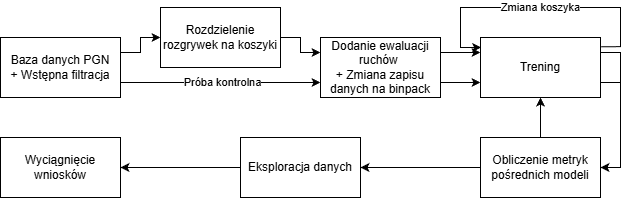
\includegraphics[width=0.7\linewidth]{workflow.png}
    \caption{Schemat przepływu danych oraz architektury eksperymentu badawczego.}
    \label{fig:workflow}
\end{figure}

Cały proces eksperymentu składa się z następujących kroków:

\begin{enumerate}
    \item \textbf{Przygotowanie i przefiltrowanie bazy danych PGN:} Surowe partie pobrane z serwisu Lichess poddawane są czyszczeniu.
    \item \textbf{Podział na koszyki Elo oraz transformacja danych:} W wariancie badawczym przefiltrowane partie rozdzielane są na osobne grupy reprezentujące rosnące przedziały rankingowe (po 2~miliony partii na koszyk). W przypadku próby kontrolnej partie z różnych przedziałów są losowo wymieszane w ramach jednego zbioru. Następnie dane są ewaluowane i konwertowane do binarnego formatu \texttt{.binpack}. Analogiczny proces jest również wykonany dla danych walidacyjnych (po 200~tysięcy partii na koszyk).
    \item \textbf{Trening sieci neuronowej:} Uczenie odbywa się przy użyciu biblioteki \texttt{nnue-pytorch}. W wariancie badawczym model po osiągnięciu założonej liczby epok (100 epok na koszyk) przechodzi do kolejnego zbiornika PGN, kontynuując naukę z ostatniego punktu kontrolnego (\textit{checkpoint}) poprzedniego etapu.
    \item \textbf{Obliczenie metryk pośrednich i ewaluacja:} Po stworzeniu plików checkpoint przez skrypt treningowy wykonuję serializację zapisanych wag sieci do plików \texttt{.nnue}, następnie uruchamiam skrypt run\_tournament który automatycznie porównuje ze sobą stworzone sieci na różne sposoby wykorzystując do tego narzędzie \texttt{cutechess-cli}
    \item \textbf{Eksploracja danych i wnioskowanie:} Zgromadzone informacje o procesie uczenia jak i późniejszej ewaluacji silników poddane zostaną analizie z której wyciągnę wnioski w celu weryfikacji postawionych hipotez.
\end{enumerate}

\section{Parametry treningu}

Trening sieci realizowano z wykorzystaniem frameworka \texttt{nnue-pytorch} (opartego na \texttt{PyTorch Lightning}). Zastosowano spójny zestaw hiperparametrów dla wszystkich analizowanych wariantów eksperymentalnych:

\begin{itemize}
    \item \textbf{Reprezentacja cech (\textit{Feature Set}):} Zastosowałem układ \textit{HalfKAv2\_hm\string^}. Ten format reprezentuje rzadkie wektory uwzględniające relacje między własnym i obcym królem a całą resztą bierek, gdzie pozycje dzielone są na 8 niezależnych koszyków \textit{layer-stacks} w zależności od obecnej fazy gry (liczby figur pozostałych na stole).
    \item \textbf{Wielkość wsadu (\textit{Batch Size}):} Trening prowadzono z rozmiarem wsadu równym $16\,384$ pozycji. Wybór tak dużego wsadu zapewnia wysoką stabilność estymacji gradientu na kartach graficznych o dużej pamięci VRAM oraz optymalne wykorzystanie mocy obliczeniowej GPU.
    \item \textbf{Współczynnik straty (\textit{Lambda}):} Ustawiając parametr $\lambda = 0{,}3$, precyzyjnie uregulowałem stosunek znaczenia oceny między dwoma różnymi ujęciami błędu. Znaczyło to, że 30\% docelowej wartości wag dla funkcji straty uwarunkowałem na idealnej, statycznej ocenie silnika Stockfish nałożonej na historyczną pozycję gry, podczas gdy pozostałe 70\% podyktowane było bezpośrednim rezultatem faktycznej partii pomiędzy dwoma ludźmi pobranej z bazy Lichess. Ma to na celu skuteczne eliminowanie efektu przeuczenia się modelu (\textit{overfittingu}) na specyficzne omyłki robione przez szachistów na danym pułapie Elo.
    \item \textbf{Liczba epok i harmonogram:} Dla każdego koszyka rankingowego zaplanowano po 100 epok uczenia (co sumarycznie dla 3 koszyków przekłada się na 300 epok i około 50--80 godzin ciągłych obliczeń). Zapis stanu sieci (\textit{checkpoint}) wykonywany był co 10 epok (\texttt{--network-save-period 10}).
\end{itemize}

Przykładowe uruchomienie procesu uczenia wewnątrz środowiska przedstawia poniższy listing:

\begin{lstlisting}[language=bash, caption=Polecenie uruchamiające proces uczenia na pierwszym koszyku Elo]
python train.py \
    clean_1200_under_2mil.binpack \
    --validation-datasets clean_1200_under_200k.binpack \
    --default-root-dir /data/trained_nets/ \
    --gpus 0 \
    --threads 4 \
    --batch-size 16384 \
    --lambda 0.3 \
    --max-epochs 100 \
    --features "HalfKAv2_hm^" \
    --network-save-period 10
\end{lstlisting}

\section{Infrastruktura obliczeniowa}

Ze względu na skomplikowane zależności bibliotek (\texttt{PyTorch}, \texttt{CUDA}/\texttt{ROCm}, \texttt{PyTorch Lightning}) oraz wymóg odizolowania środowiska uruchomieniowego, cały proces uczenia oraz serializacji modeli został wykonany wewnątrz kontenera \textbf{Docker}, którego plik uruchomieniowy stanowi część projektu nnue-pytorch, do których dodałem swoje modyfikacje aby współpracował z posiadaną przeze mnie kartą graficzną.

Środowisko sprzętowo-programowe wykorzystane w eksperymencie obejmowało:

\begin{itemize}
    \item \textbf{Jednostkę obliczeniową (GPU):} Karta graficzna AMD Radeon RX 6800 XT z 16 GB pamięci VRAM, wykorzystująca przyspieszenie sprzętowe w środowisku sterowników ROCm (przekazywanie urządzeń \texttt{/dev/kfd} oraz \texttt{/dev/dri} do kontenera).
    \item \textbf{Konfigurację kontenera:} Kontener uruchamiano z prawami dostępu do grup systemowych \texttt{render} oraz \texttt{video}, z nieskończonym limitem blokowania pamięci (\texttt{--ulimit memlock=-1}) oraz zwiększonym rozmiarem stosu, co wyeliminowało wąskie gardła podczas przesyłania dużych zbiorów \texttt{.binpack} z dysku do pamięci GPU.
    \item \textbf{Środowisko wykonawcze (Python):} Środowisko wewnątrz kontenera zostało dostosowane aby wszystkie wersje pakietów Python były spójne z kombinacją wszystkich zależności i wymagań.
\end{itemize}

\chapter{Ewaluacja i wyniki}

\section{Metryki oceny}

\begin{itemize}
    \item Ranking Elo (turnieje Cutechess).
    \item Zgodność z ruchami ludzkimi (Human-like Index).
    \item Krzywe funkcji straty (Loss Curve).
\end{itemize}

\section{Wyniki eksperymentu}

Przy użyciu napisanego skryptu ewaluacyjnego \texttt{run\_tournament\_nnue.py} zebrałem szczegółowe statystyki z przeprowadzonych turniejów. Z logów zarejestrowanych w formacie JSON wynikło jasno, że wchodząc w kolejne wyższe pułapy testowe (ograniczanego na poziomie 1350, 1500 oraz 1800 Elo bazowego silnika Stockfish), z każdą kolejną epoką mój silnik notował powolny, ale zauważalny trend wzrostowy. Zbiegał on od ogromnych ujemnych marginesów błędu na starcie w kierunku bezpieczniejszej, wygrywającej gry przeciwko kotwicom pomiarowym.

Na Rysunku~\ref{fig:elo_cumulative} przedstawiono skumulowany postęp siły gry (wartość Elo) w kolejnych epokach treningowych dla grupy kontrolnej (uczonej na wymieszanych danych) oraz grupy badawczej (poddanej procesowi \textit{curriculum learning}). Jak można zauważyć, model kontrolny wykazuje stosunkowo płynny przyrost siły na przestrzeni całego treningu. Z kolei w przypadku modelu badawczego postęp ten charakteryzuje się znacznie wyższą wariancją w obrębie danego koszyka.

\begin{figure}[htbp]
    \centering
    \begin{subfigure}[b]{0.48\textwidth}
        \centering
        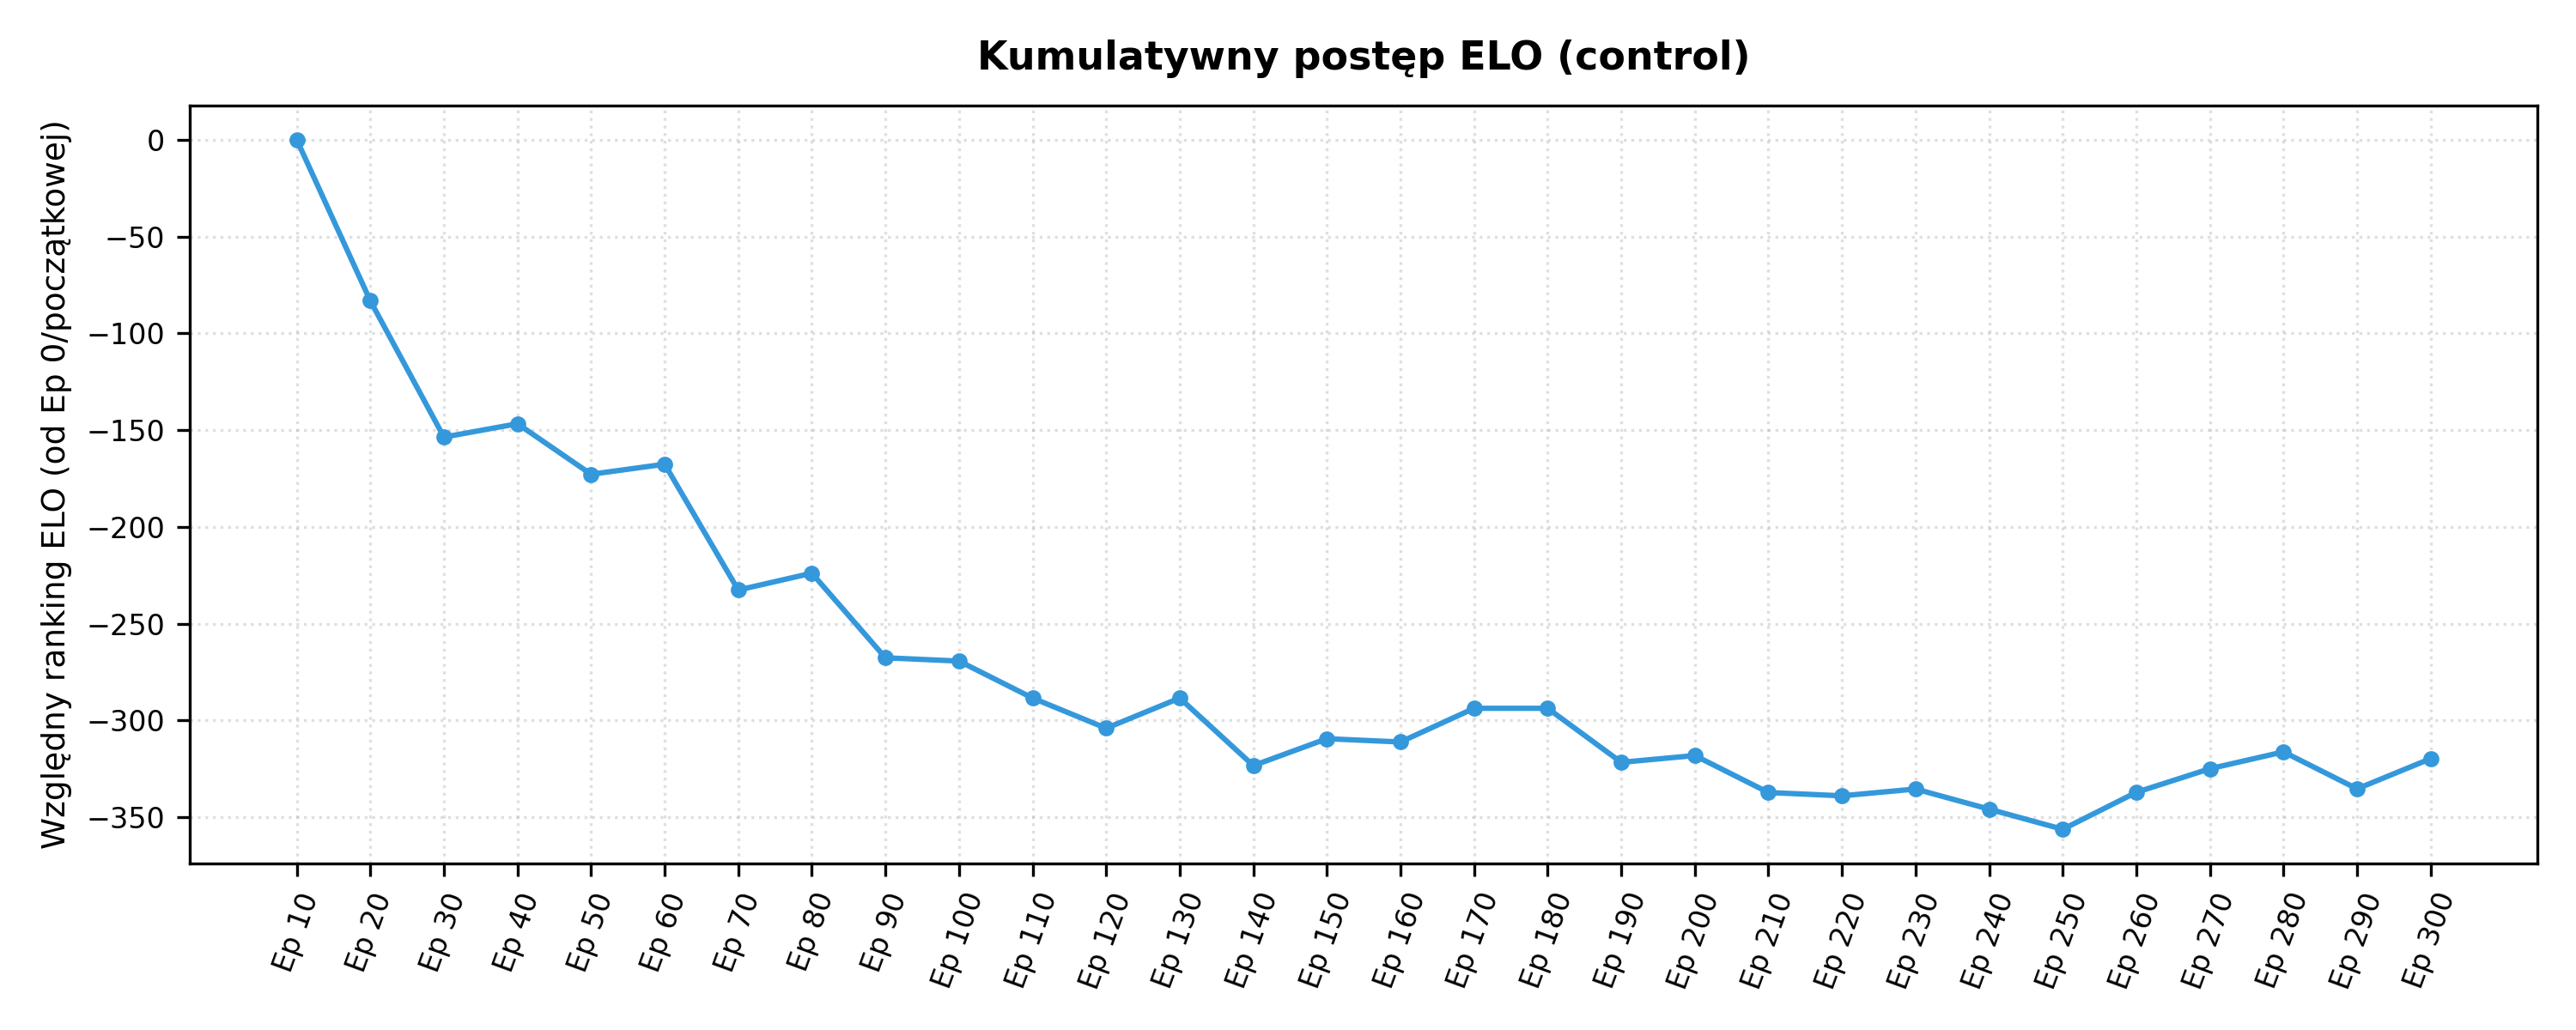
\includegraphics[width=\textwidth]{elo_cumulative_progression_control.png}
        \caption{Grupa kontrolna (brak zmiany koszyków)}
        \label{fig:elo_cumulative_control}
    \end{subfigure}
    \hfill
    \begin{subfigure}[b]{0.48\textwidth}
        \centering
        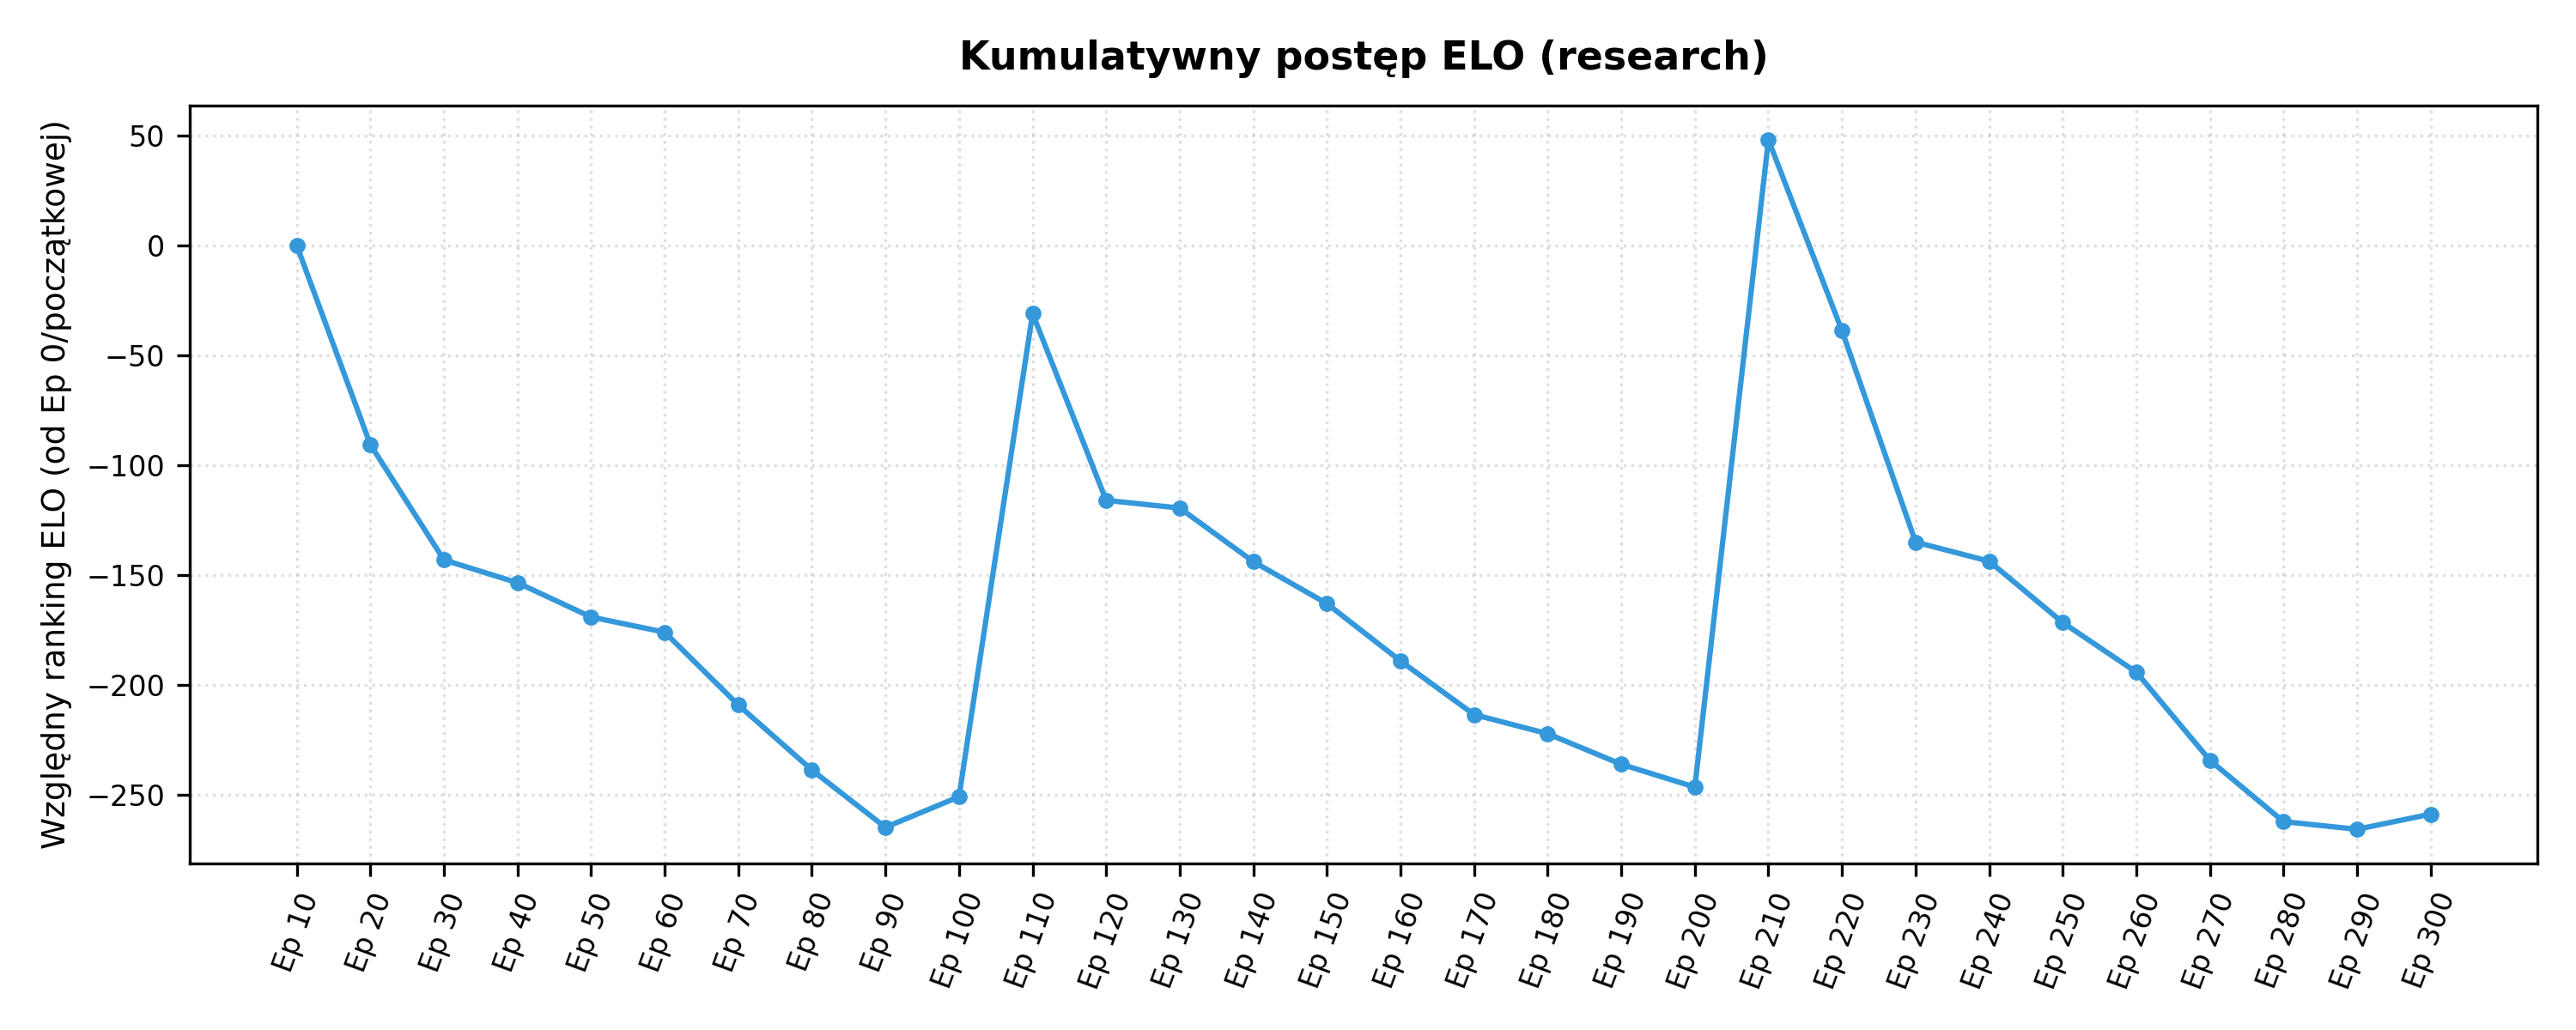
\includegraphics[width=\textwidth]{elo_cumulative_progression_research.png}
        \caption{Grupa badawcza (zmiana koszyków co 100 epok)}
        \label{fig:elo_cumulative_research}
    \end{subfigure}
    \caption{Skumulowany postęp Elo na przestrzeni epok.}
    \label{fig:elo_cumulative}
\end{figure}

W celu lepszego zrozumienia zachowania modelu badawczego w momentach tuż przed zmianą zestawu danych uczących, wygenerowano dodatkowe wykresy ograniczające analizę do trzech kluczowych momentów -- punktów zapisu silnika odpowiadających ostatnim iteracjom w każdym koszyku. Rysunek~\ref{fig:elo_research_3} uwydatnia, jak kształtowała się siła gry dla poszczególnych silników (rozpatrywanych jako 3 oddzielne sieci badane w tym samym czasie) podczas tych weryfikacji.

\begin{figure}[htbp]
    \centering
    \begin{subfigure}[b]{0.48\textwidth}
        \centering
        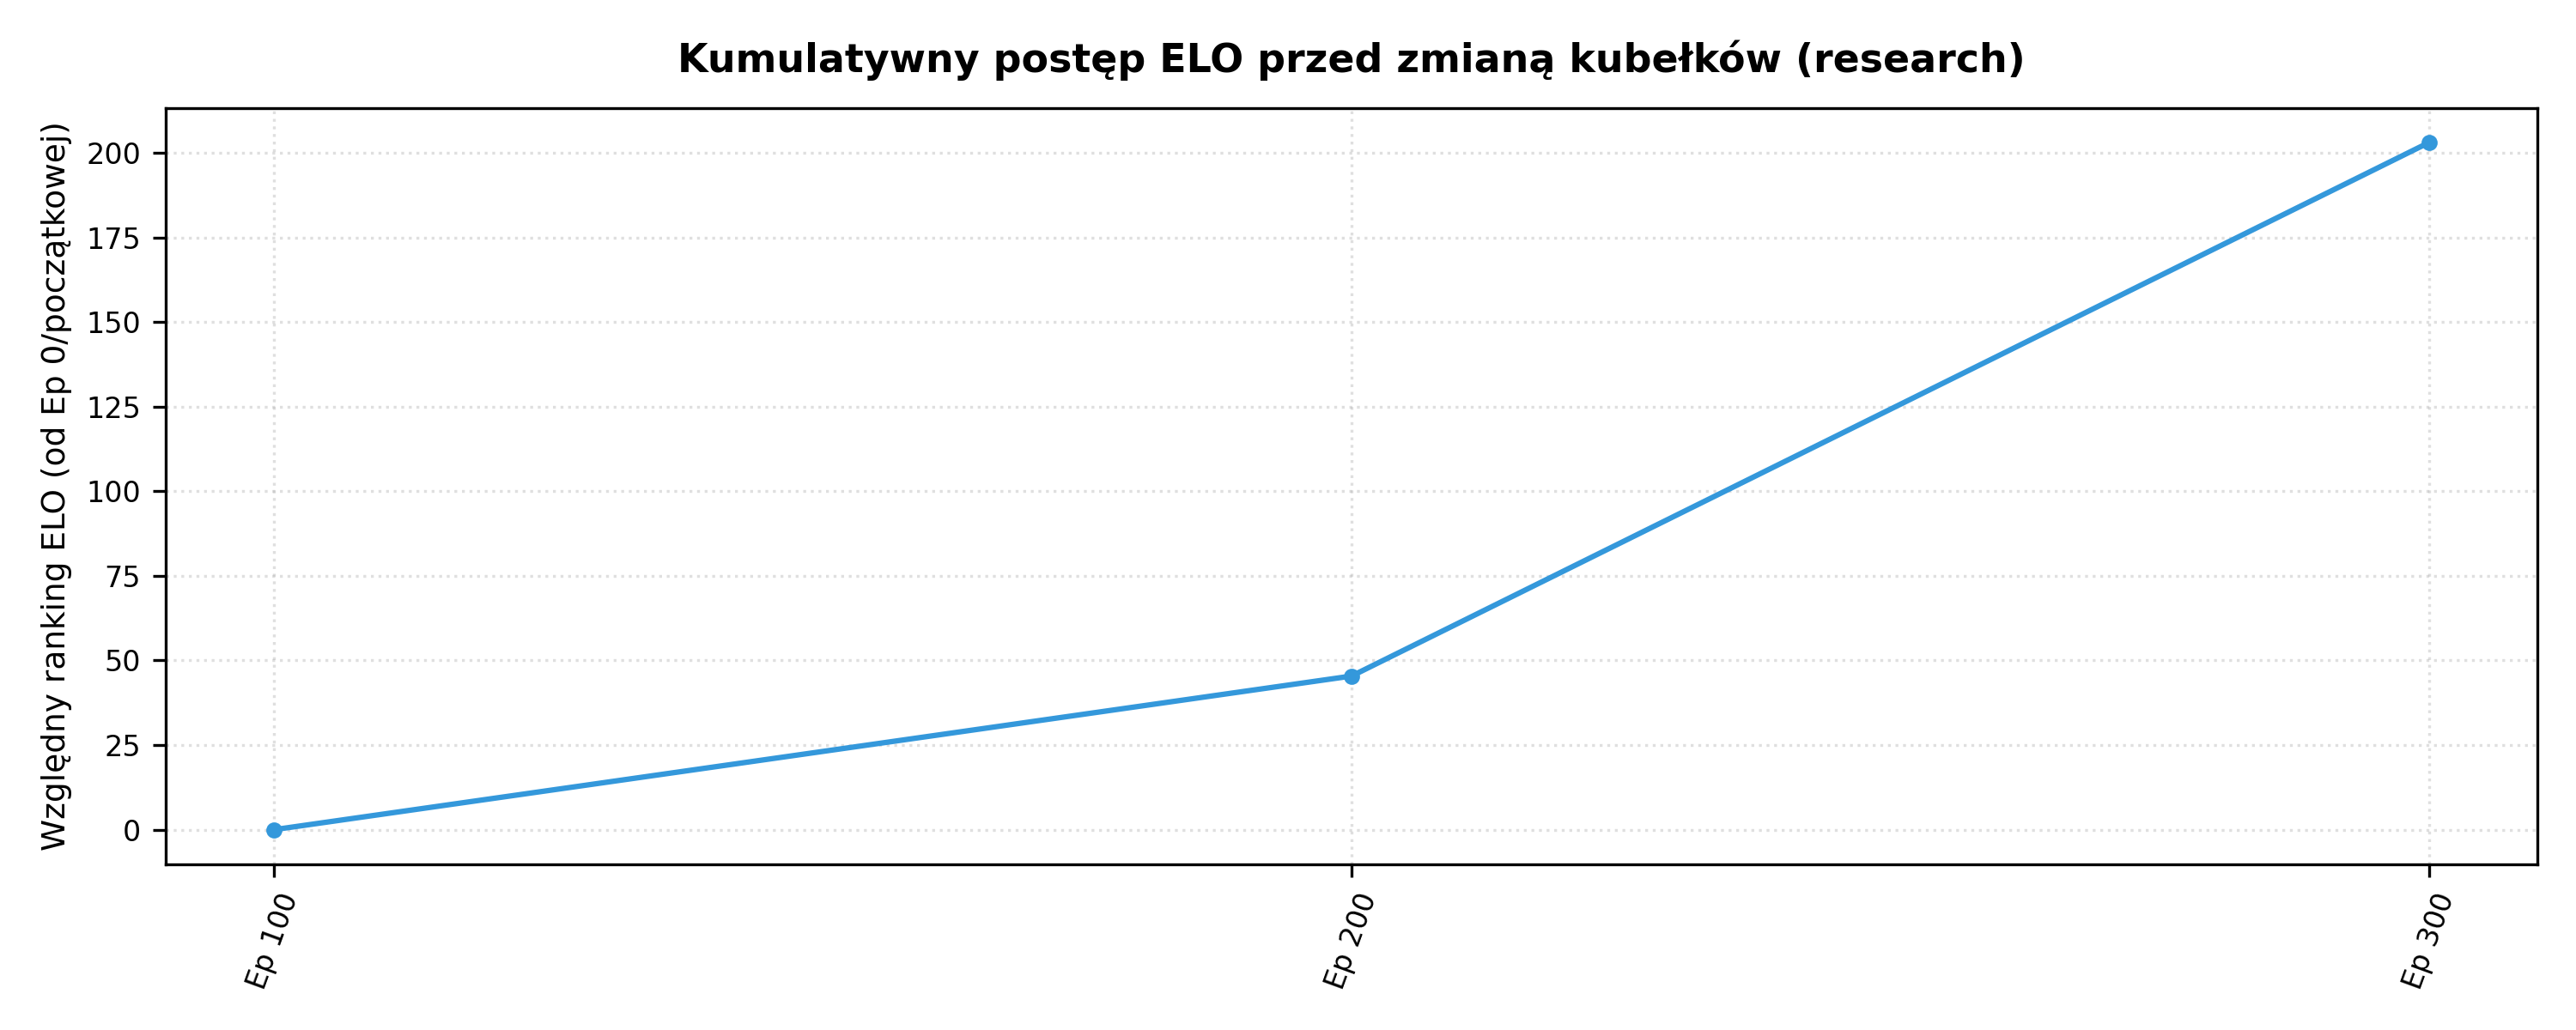
\includegraphics[width=\textwidth]{elo_cumulative_progression_research_3.png}
        \caption{Skumulowane Elo dla 3 silników przed zmianą danych}
        \label{fig:elo_cumulative_research_3}
    \end{subfigure}
    \hfill
    \begin{subfigure}[b]{0.48\textwidth}
        \centering
        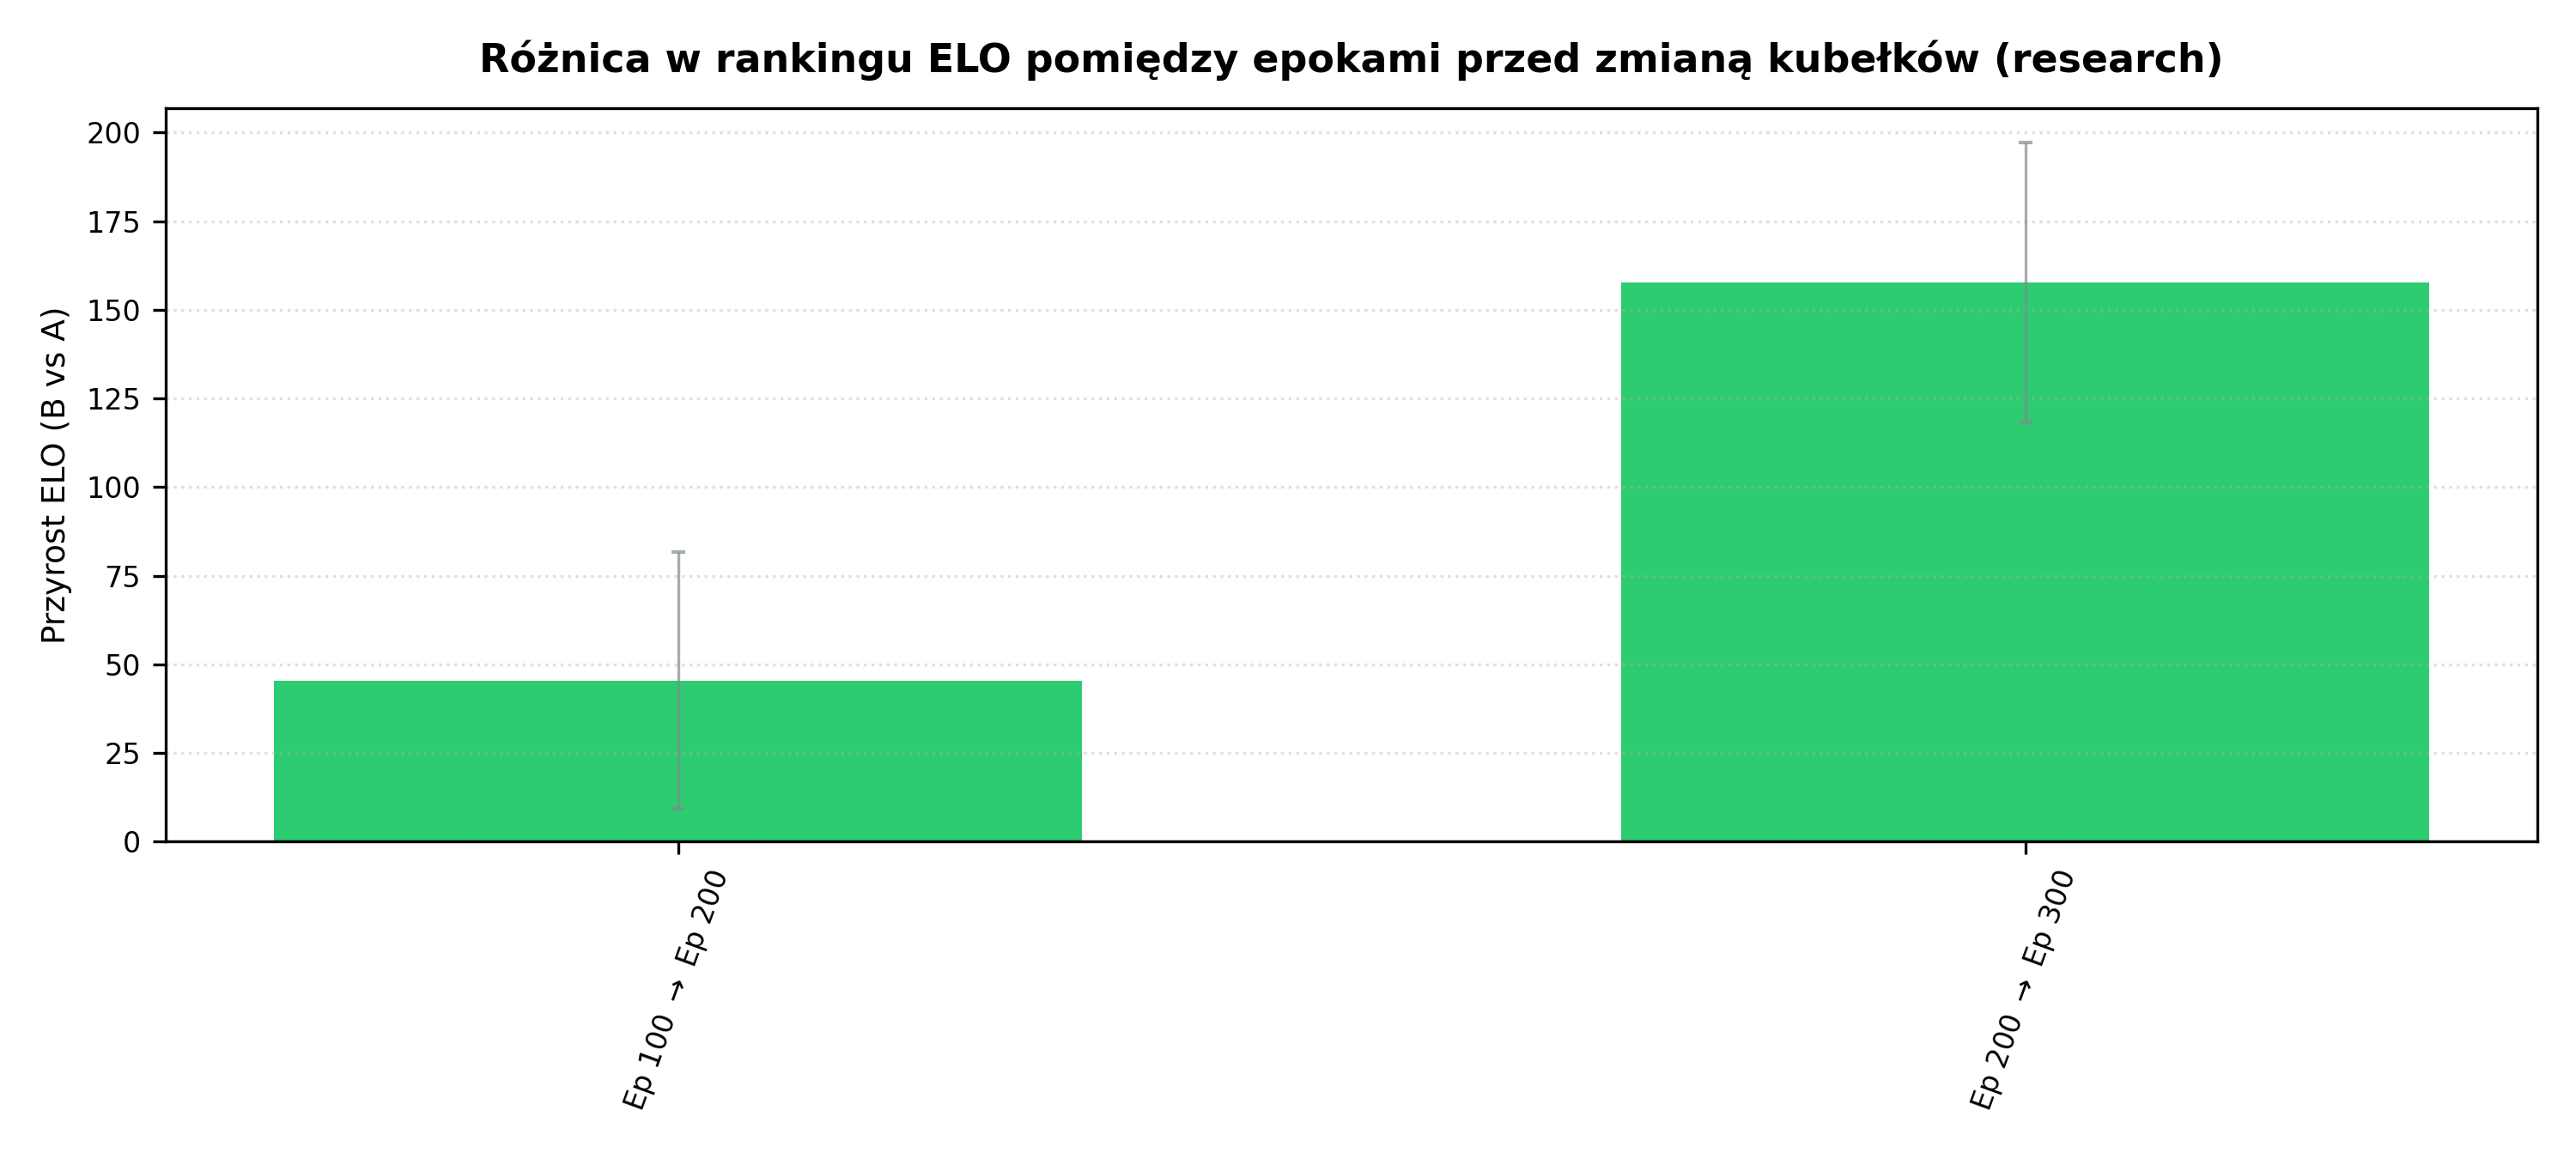
\includegraphics[width=\textwidth]{elo_differences_research_3.png}
        \caption{Różnice Elo dla 3 silników przed zmianą danych}
        \label{fig:elo_differences_research_3}
    \end{subfigure}
    \caption{Wykresy dla grupy badawczej uwzględniające wyniki ewaluacji z udziałem 3 silników, badające stan wag bezpośrednio przed zmianą danych treningowych (ostatnie wersje z poszczególnych przedziałów).}
    \label{fig:elo_research_3}
\end{figure}

Kolejnym niezwykle interesującym aspektem są przyrosty (bądź spadki) siły gry pomiędzy kolejnymi ewaluacjami turniejowymi. Na Rysunku~\ref{fig:elo_differences} zestawiono różnice punktowe Elo z pomiaru na pomiar dla obu grup, co ukazuje dynamikę i stabilność przyswajania wiedzy przez sieci.

\begin{figure}[htbp]
    \centering
    \begin{subfigure}[b]{0.48\textwidth}
        \centering
        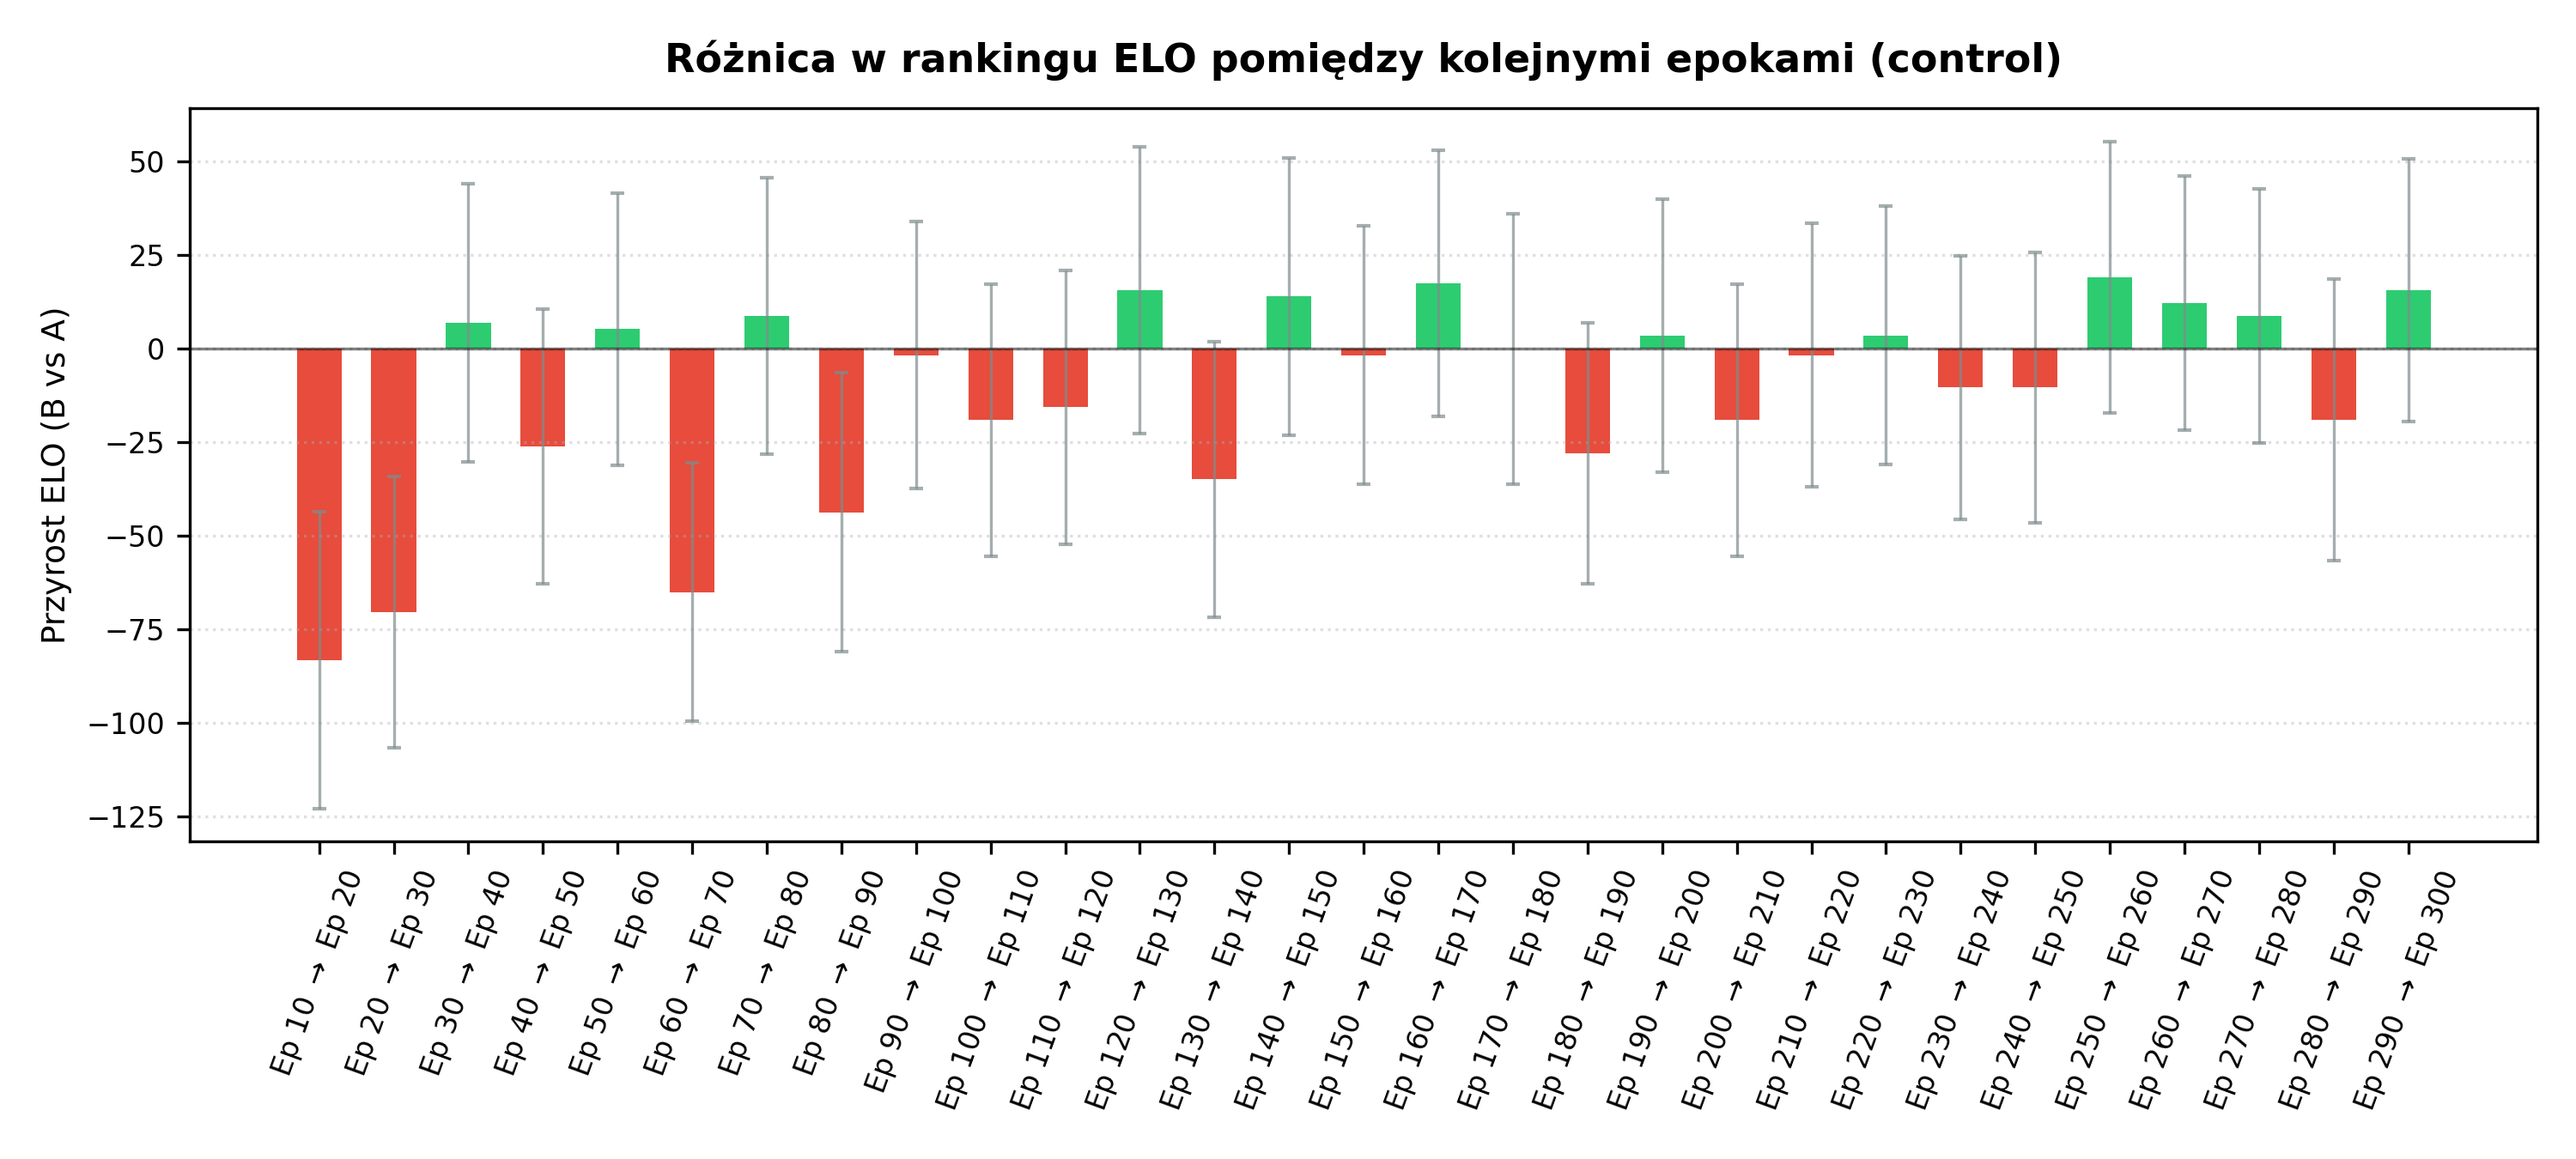
\includegraphics[width=\textwidth]{elo_differences_control.png}
        \caption{Różnice Elo -- grupa kontrolna}
        \label{fig:elo_differences_control}
    \end{subfigure}
    \hfill
    \begin{subfigure}[b]{0.48\textwidth}
        \centering
        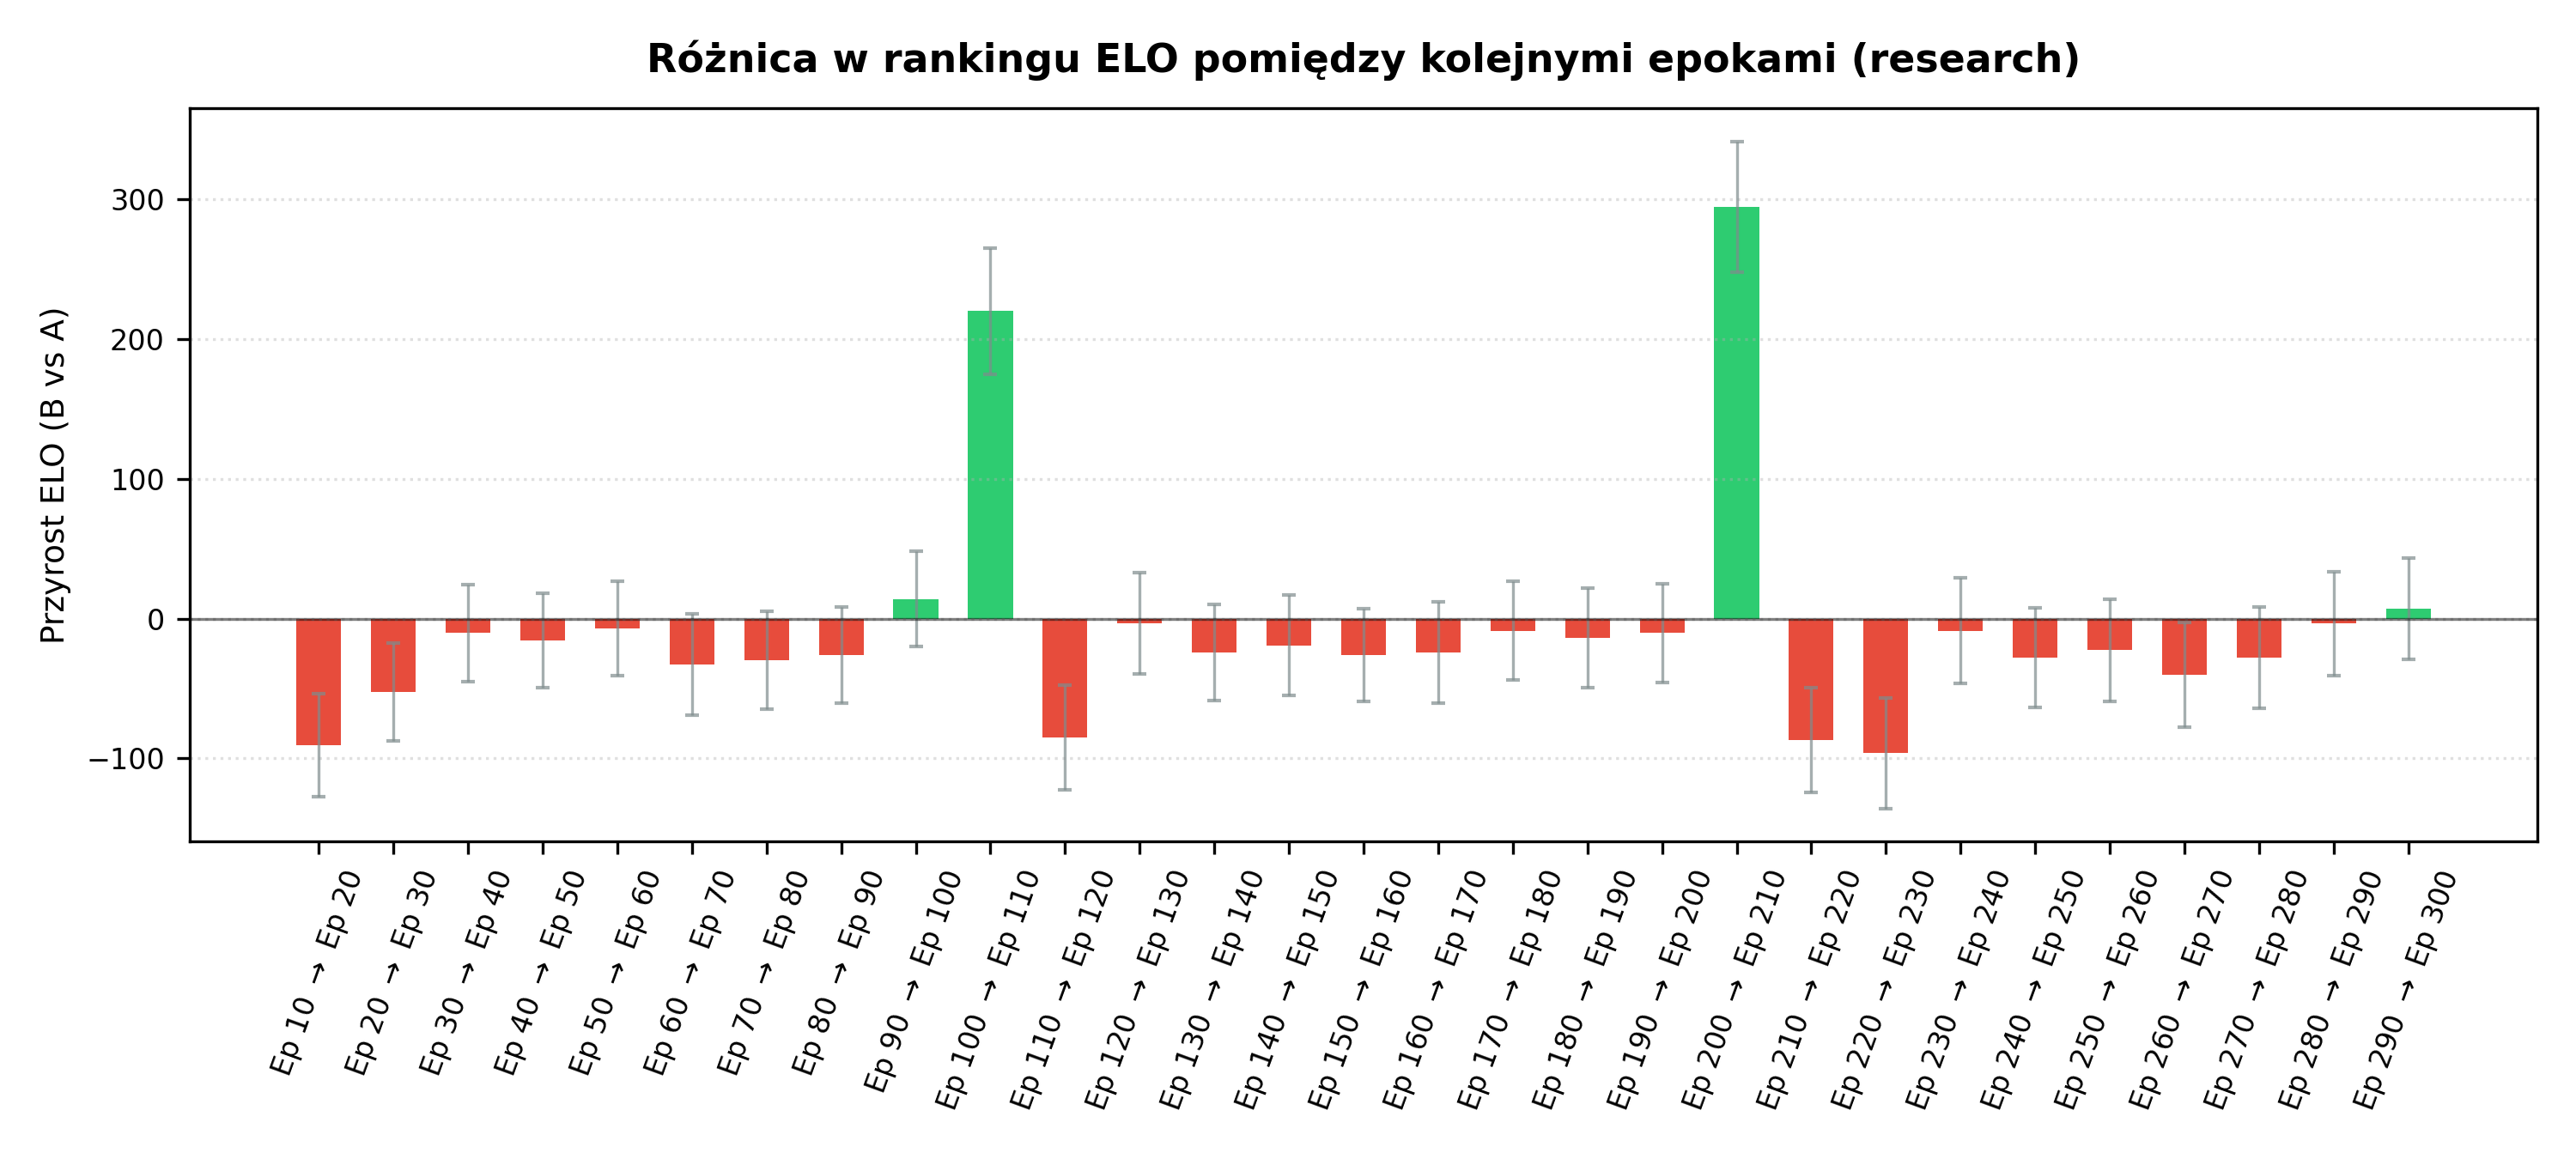
\includegraphics[width=\textwidth]{elo_differences_research.png}
        \caption{Różnice Elo -- grupa badawcza}
        \label{fig:elo_differences_research}
    \end{subfigure}
    \caption{Dynamika zmian (różnica Elo z epoki na epokę) w trakcie procesu uczenia.}
    \label{fig:elo_differences}
\end{figure}

\subsection{Zgodność z ruchami ludzkimi (Move Matching)}

Weryfikację założenia, że silnik po procesie \textit{curriculum learning} będzie grać w sposób bardziej zbliżony do człowieka na danym poziomie, przeprowadzono badając tzw. Human-like Index. Za pomocą autorskiego skryptu zestawiono odpowiedzi silnika na zadane pozycje (przeszukiwanie o głębokości równej 1) z faktycznymi posunięciami wykonanymi przez człowieka w partiach historycznych z przedziałów Elo użytych w danym koszyku.

Na Rysunku~\ref{fig:human_like_comparison} zobrazowano procent zgodności odpowiedzi silnika z posunięciami ludzkimi w trakcie trwania treningu. Należy zaznaczyć, że podczas testów grupy badawczej zbiór testowy PGN ulegał zmianie w okolicach epoki 100 oraz 200, odpowiadając charakterystyce wczytywanego w danym momencie koszyka (odpowiednio dla poziomów Elo: 1200, 1500 oraz 1800). Z kolei w grupie kontrolnej model badany był bez przerwy na całym przekroju poziomów (0-1800).

\begin{figure}[htbp]
    \centering
    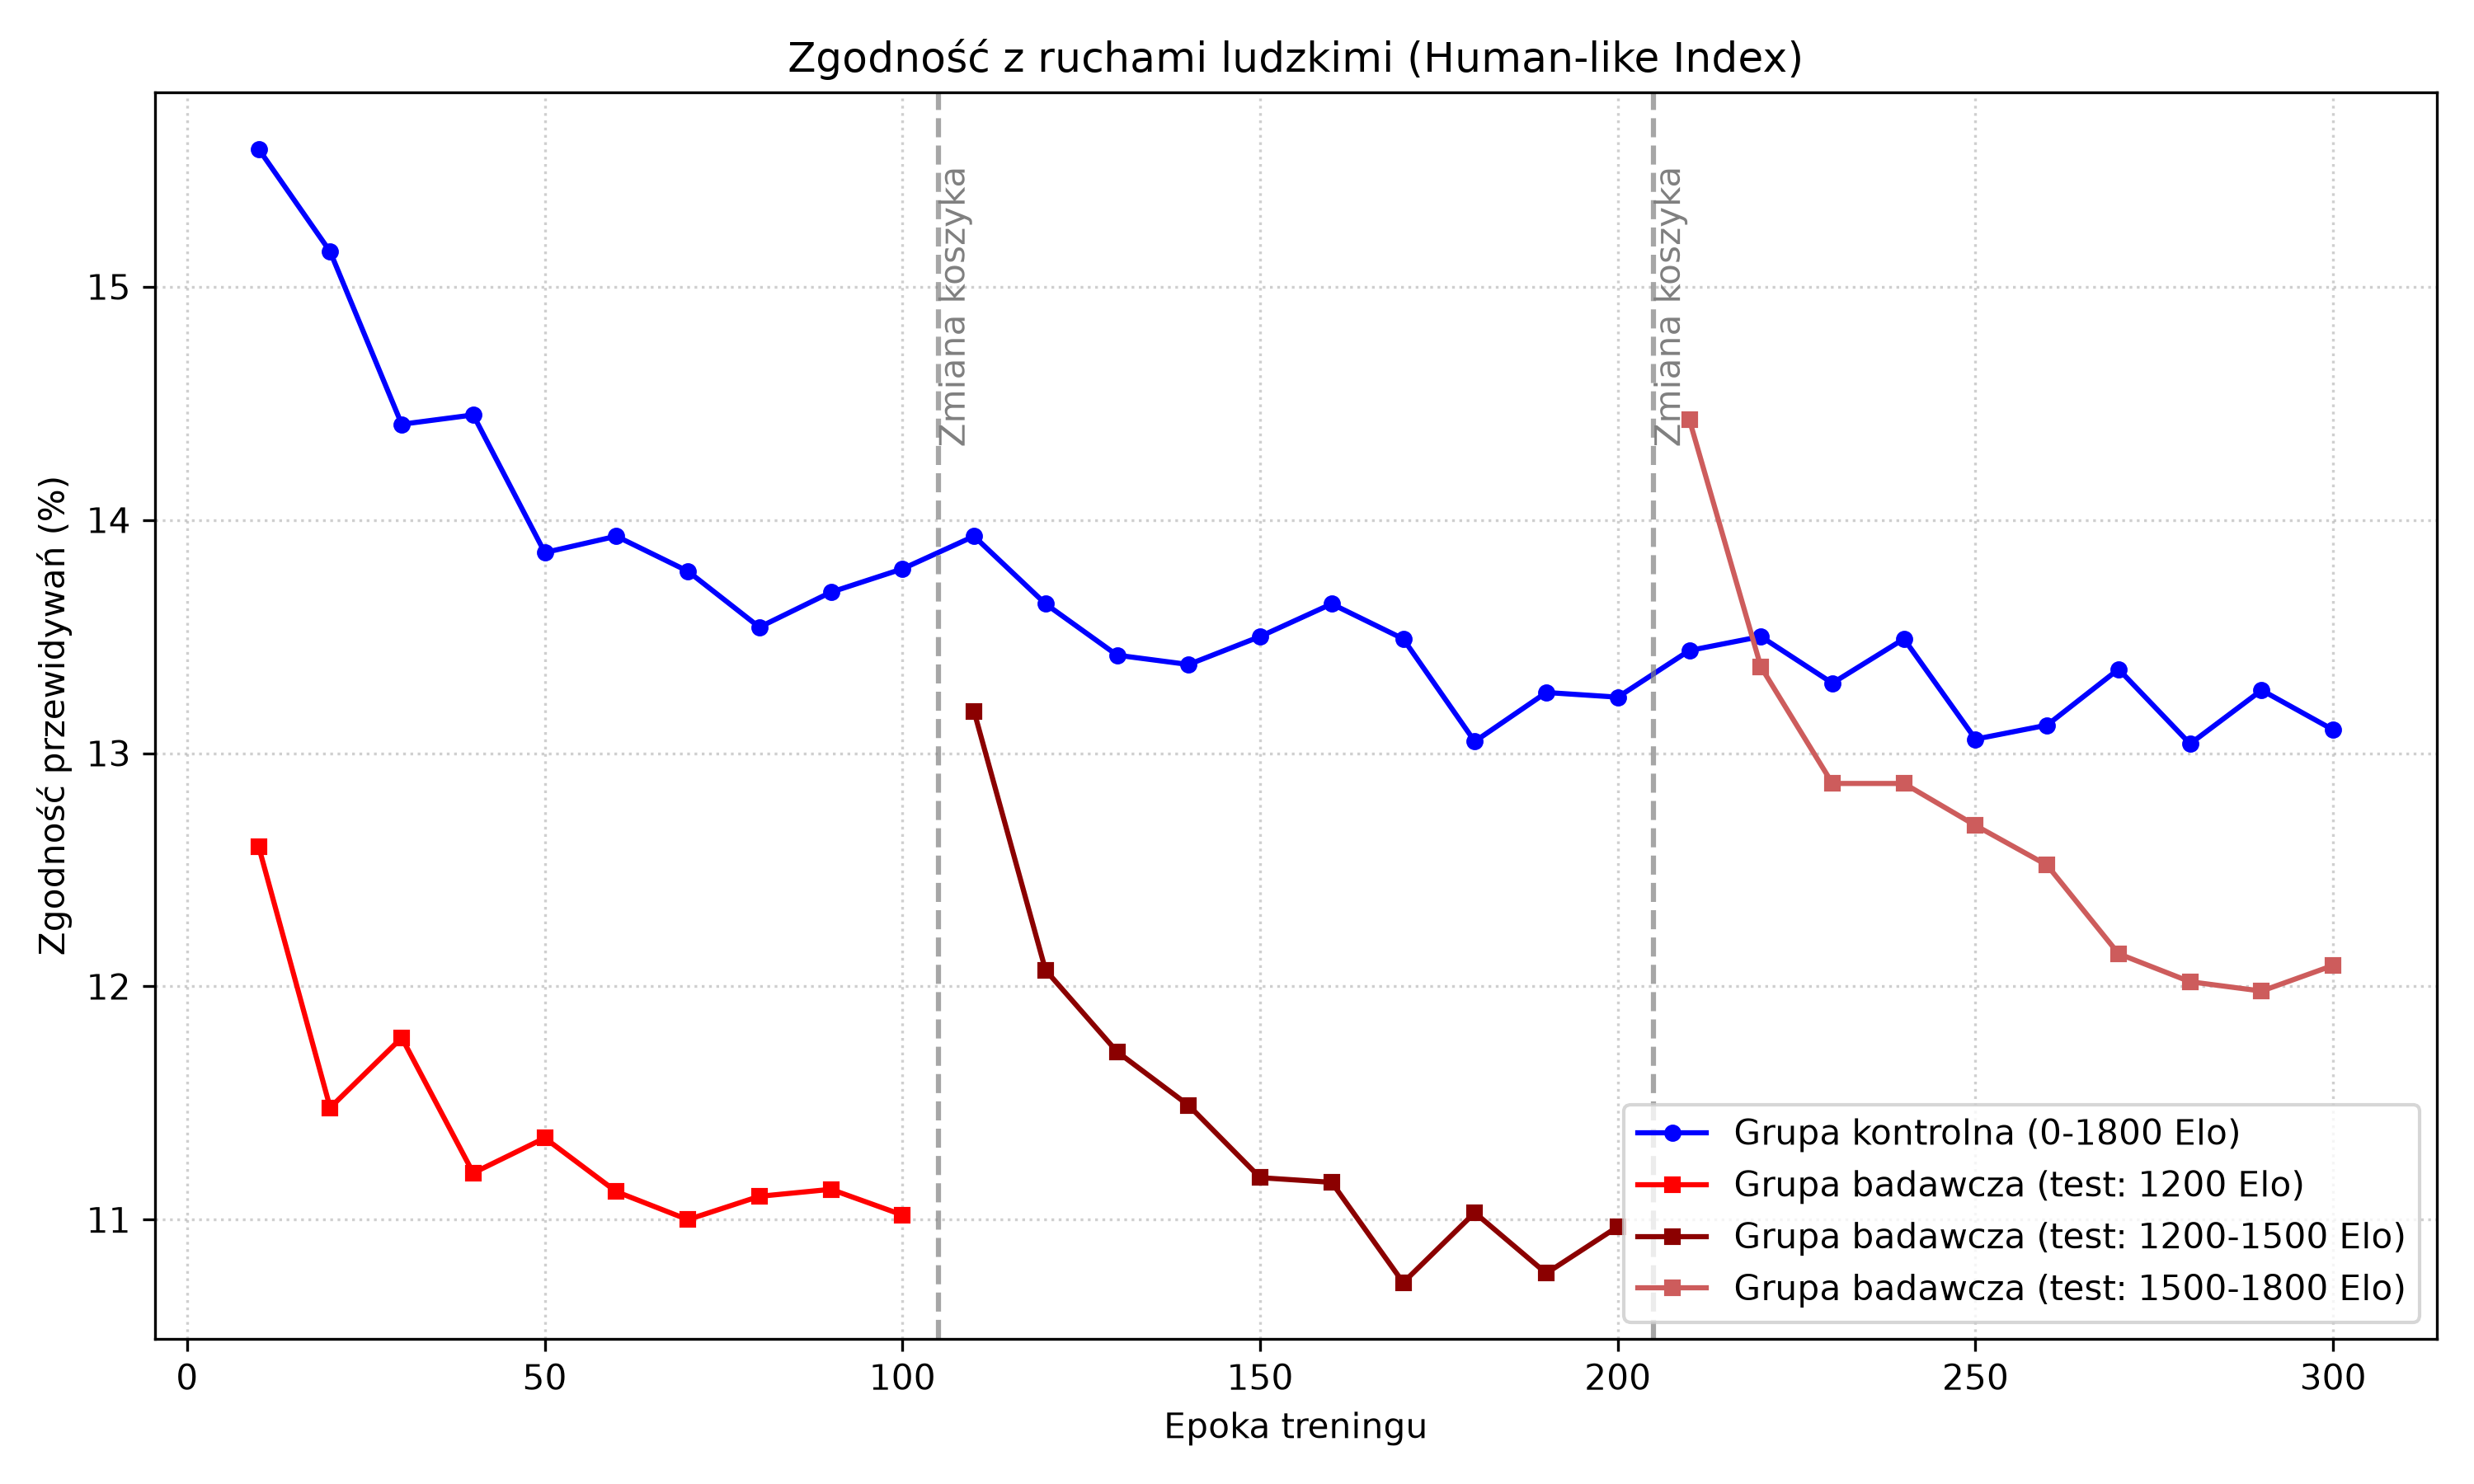
\includegraphics[width=\textwidth]{human_like_comparison.png}
    \caption{Skuteczność przewidywań ludzkich ruchów w kolejnych epokach treningu.}
    \label{fig:human_like_comparison}
\end{figure}

Z zaprezentowanych wyników jednoznacznie wynika, że w miarę upływu treningu wewnątrz każdego z koszyków, zgodność z ludzkimi zagraniami sukcesywnie spada. Dzieje się tak, ponieważ sieć coraz lepiej optymalizuje statyczną wiedzę i wybiera obiektywnie lepsze, "maszynowe" zagrania, oduczając się suboptymalnych zagrań typowych dla amatorów. Niezwykle interesujący jest jednak nagły, pionowy skok parametru Human-like Index występujący przy przejściu do kolejnego koszyka (np. tuż po epoce 100 i 200). Udowadnia on, że sieć pod wpływem nowych, lepszych jakościowo danych bardzo mocno internalizuje na chwilę "świeże" wzorce zachowań charakterystycznych dla graczy z nowego, wyższego przedziału Elo, po czym w miarę dalszej nauki znów zaczyna je optymalizować na rzecz poprawności czysto matematycznej. 

Co więcej, najwyższy pułap dopasowania w grupie kontrolnej (ponad 15\% względem zbioru 0-1800) znacząco przewyższa początkowe wskaźniki modelu badawczego z pierwszego etapu, co wskazuje, że samo zjawisko \textit{curriculum learning} nie ułatwia nauki naśladowania najsłabszych graczy i rzuca krytyczne światło na hipotezę H2 z technicznego punktu widzenia.

\section{Analiza skoków rozwojowych}

Sprawdziłem, w jakim stopniu zmiana zbioru z danymi najsłabszych szachistów na dane uchodzące za bardziej złożone, pochodzące z puli mistrzowskiej (gdzie Elo rośnie diametralnie) wpływała na siłę silnika i proces jego optymalizacji. Na Rysunku~\ref{fig:loss_comparison} przedstawiono krzywe funkcji straty dla obu głównych wariantów. Zestawiając je ze sobą, odnotowałem na wykresie grupy badawczej niespodziewane, gwałtowne piki (\textit{Loss Spikes}) występujące dokładnie w momentach zmiany zestawu uczącego (w okolicach epoki 100 oraz 200). Analiza logów z treningu pokazała, że zmienność mikroszumu od ogólnego trendu (\textit{Noise Volatility}) podskoczyła drastycznie o 81\% w chwili zmiany bazy danych w porównaniu z gładkimi spadkami obserwowanymi na wykresie próby kontrolnej (na której wymieszałem dane losowo ze wszystkich poziomów rankingu), co uderzyło we wskaźnik całkowitej zmienności błędu wzrostem o 147\%. 

\begin{figure}[htbp]
    \centering
    \begin{subfigure}[b]{0.48\textwidth}
        \centering
        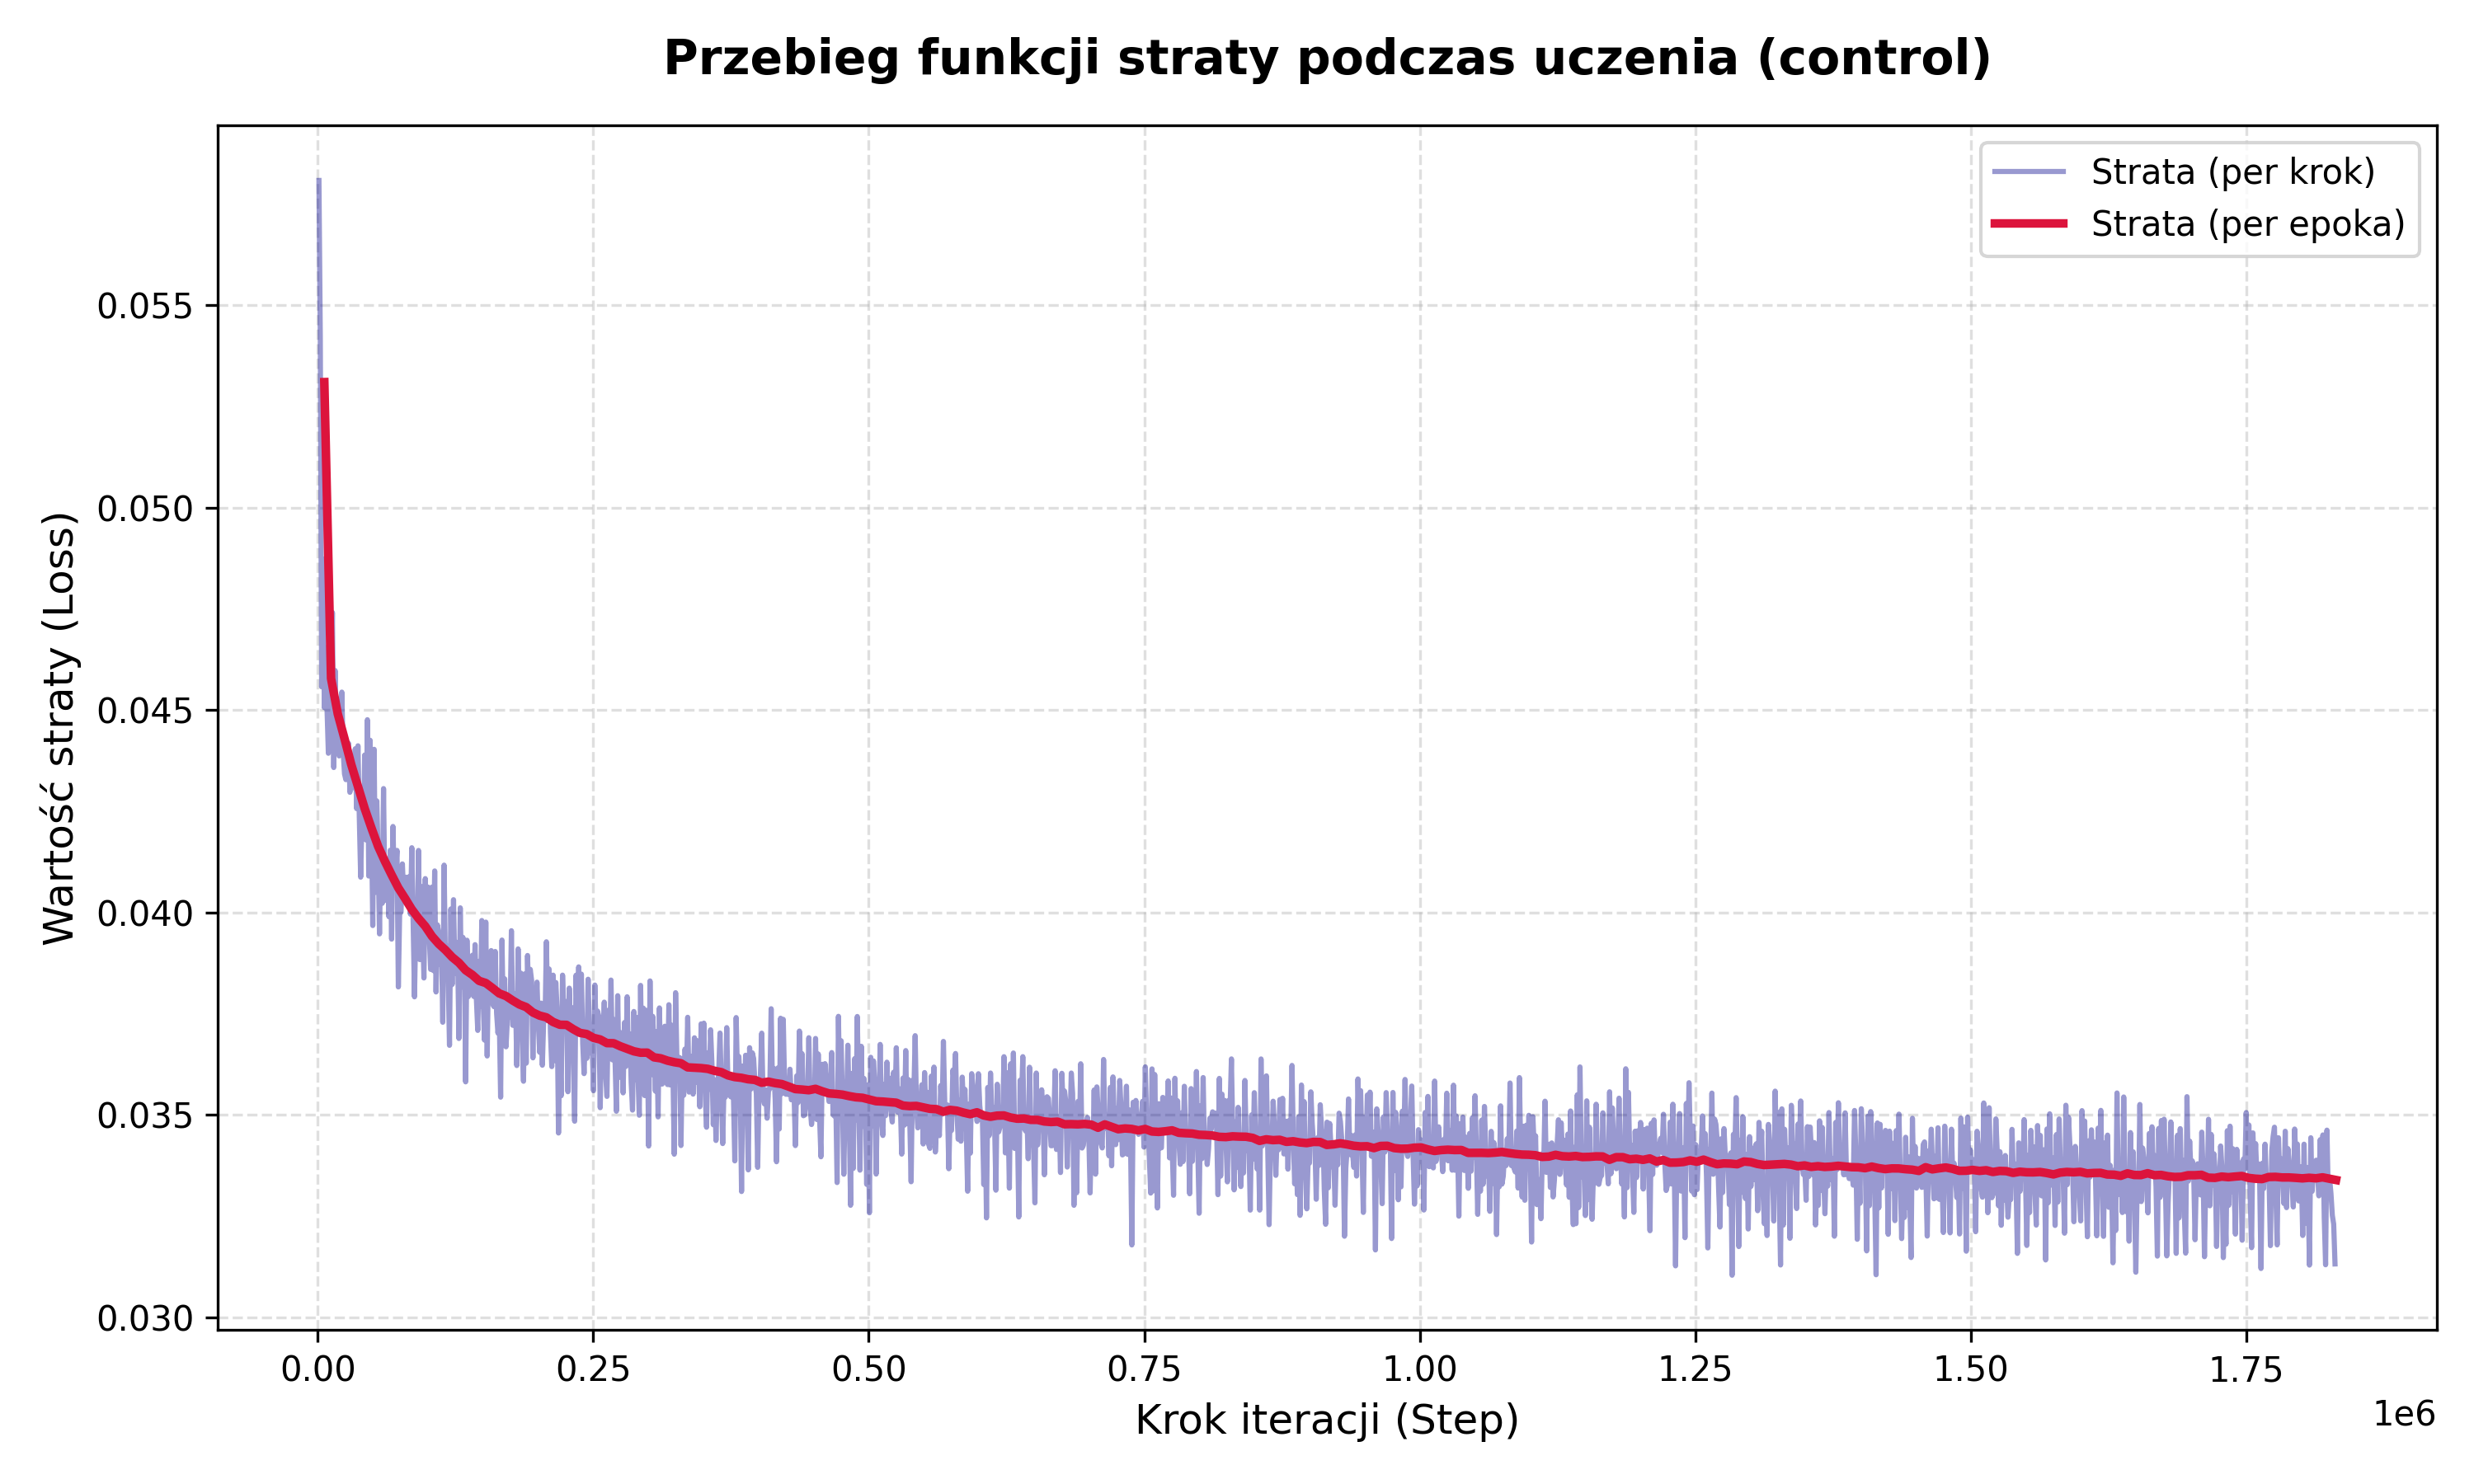
\includegraphics[width=\textwidth]{graph_control.png}
        \caption{Krzywa funkcji straty -- grupa kontrolna}
        \label{fig:loss_control}
    \end{subfigure}
    \hfill
    \begin{subfigure}[b]{0.48\textwidth}
        \centering
        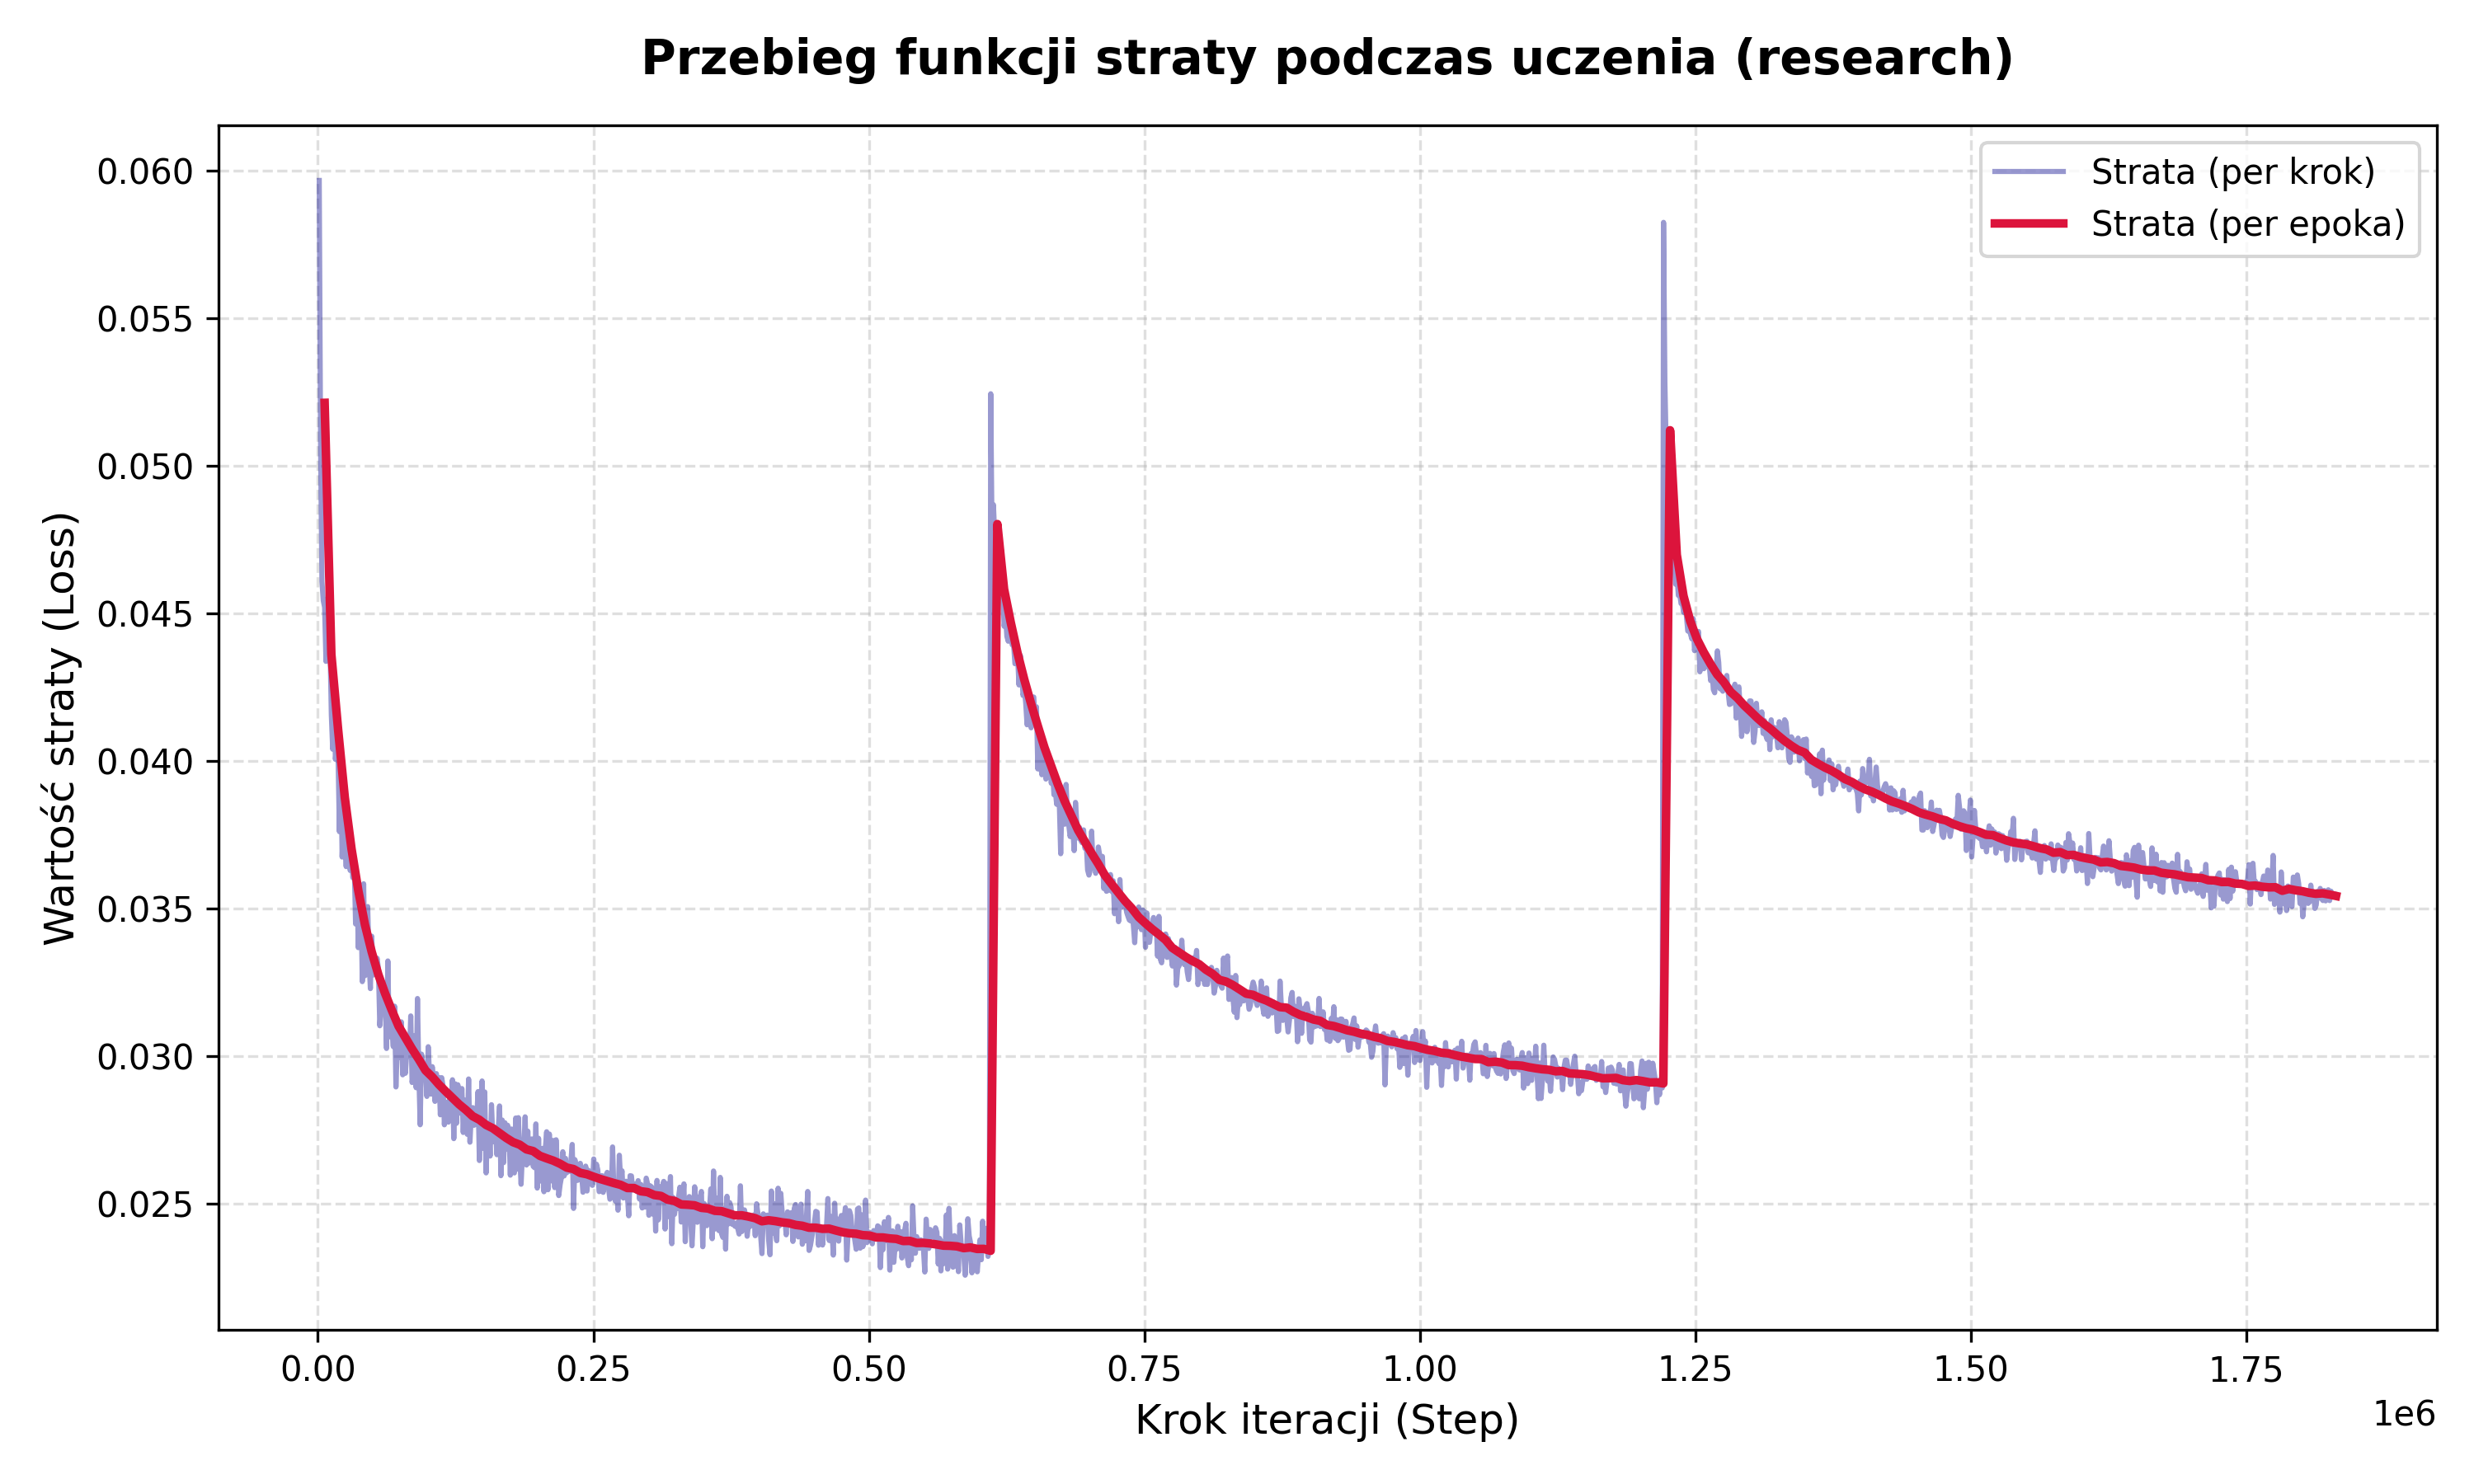
\includegraphics[width=\textwidth]{graph_research.png}
        \caption{Krzywa funkcji straty -- grupa badawcza}
        \label{fig:loss_research}
    \end{subfigure}
    \caption{Porównanie krzywych błędów treningowych z widocznymi pikami straty w momentach zmiany dystrybucji danych w grupie badawczej.}
    \label{fig:loss_comparison}
\end{figure}

Odbicie tego wstrząsu jest również widoczne na wygenerowanym wcześniej wykresie różnic Elo dla grupy badawczej (Rysunek~\ref{fig:elo_differences_research}) -- w miejscach zmiany koszyka (odpowiadających epokom granicznym) można zaobserwować wychylenia i chwilową niestabilność przyrostów punktowych w porównaniu do dużo mniejszych amplitud w grupie kontrolnej. Model tracił krótkotrwale spójność, doznając wstrząsu. Winowajcą nie był wyższy poziom szachów, ale czysto koncepcyjny dla architektur neuronowych proces szoku znanego jako \textit{Co-Domain Shift}.

\chapter{Wnioski}

\section{Weryfikacja hipotez}

Na podstawie wyciągniętych wniosków z analizy krzywych, zaprezentowanych na Rysunkach \ref{fig:elo_cumulative} i \ref{fig:elo_differences}, zdecydowałem się obalić postawioną na wstępie hipotezę \textbf{H1}. Okazało się, że podawanie bardzo słabych pod względem taktycznym gier na samym początku nauki wcale jej drastycznie nie stymulowało ani nie przyspieszało. Zmuszanie sieci do zmiany progu w górę w trybie zorganizowanego Curriculum Learning podcinało optymalizację algorytmiczną, naruszając i wyrzucając drastycznie na krótki okres jej ułożone dotychczas wagi z powodu nagłej zmiany dystrybucji danych. Jest to doskonale widoczne pod postacią nagłych wahań i skoków wariancji w modelu badawczym (szczególnie widoczne przy zmianach koszyków), w przeciwieństwie do bardziej stabilnego trendu w modelu kontrolnym.

Ewaluując odchylenia na grupie kontrolnej obaliłem również hipotezę \textbf{H3}. Zobrazował mi to dodatkowy wariant ze stworzonego eksperymentu odwróconego (uczenie od partii arcymistrzowskich w dół do słabych), którego krzywą uczenia przedstawiono na Rysunku~\ref{fig:loss_reverse}. 

\begin{figure}[htbp]
    \centering
    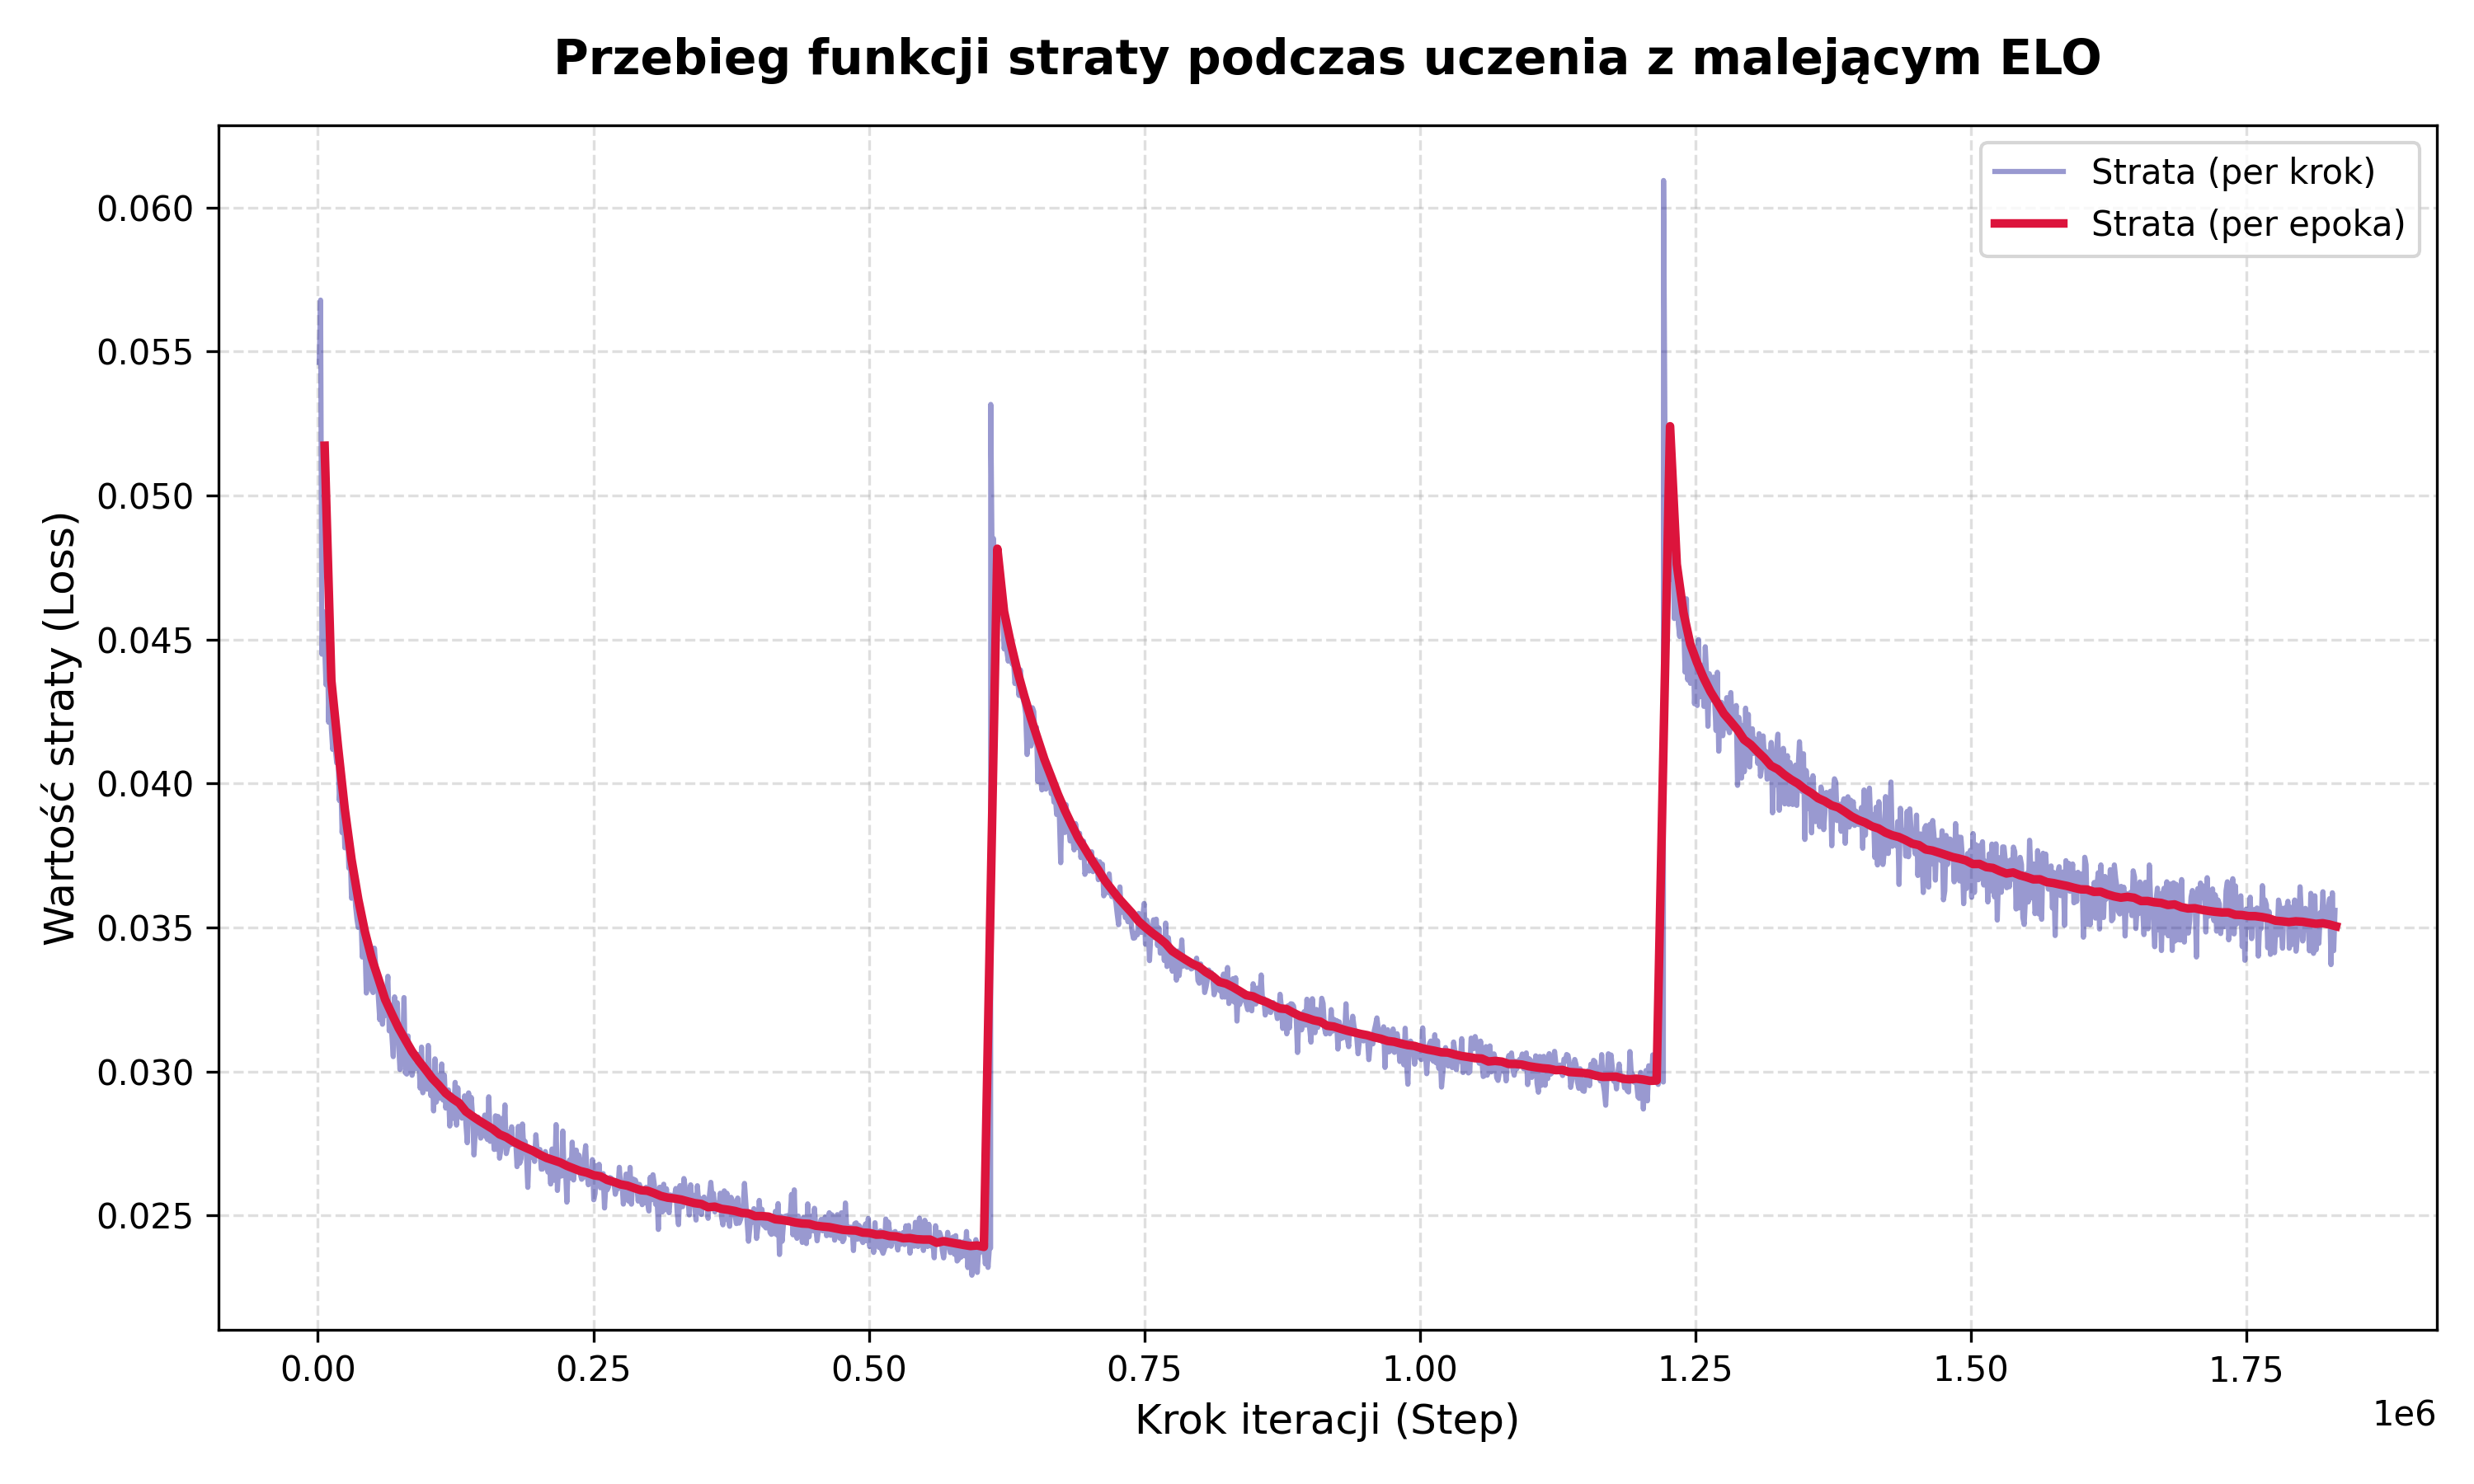
\includegraphics[width=0.7\textwidth]{graph_loss_reverse.png}
    \caption{Krzywa funkcji straty dla eksperymentu odwróconego (od trudnych do łatwych partii).}
    \label{fig:loss_reverse}
\end{figure}

Wykresy obu wariantów przeplatały się w sposób całkowicie symetryczny z różnicą zmienności Total Loss Std sięgającej na końcu zaledwie ułamkowych (niecałych czterech) procent. Podobnie jak w wariancie badawczym, tutaj również zaobserwowano analogiczne, gwałtowne piki występujące przy zmianach koszyków. Udowodniłem tym sposobem ostatecznie, że wstrząsy i skoki błędu nie są generowane przez obiektywnie "trudniejsze" partie (wyższy czy też wyimaginowanie niższy poziom logiki samych układów w datasetach), lecz uwarunkowane są wyłączenie nagłą zmianą dystrybucji danych. To właśnie owa zmiana domeny wywołuje zjawisko szoku (\textit{Co-Domain Shift}), które tak mocno destabilizuje modele trenowane z wykorzystaniem Curriculum Learning.

\section{Zastosowania praktyczne}

% Interaktywny asystent szachowy.
Pamiętając o motywacji ze wstępu mojej pracy — intencji zbudowania asystenta szachowego, który w sposób adaptacyjny douczałby się "po trochu" aktualnych posunięć przeciwko postępującym szachistom — na bazie uzyskanych wyników odradzam tego typu podejście, w którym następowałaby powolna progresywna (bądź nagła) wymiana koszyków na lepsze na produkcyjnym organizmie modelu. Wprowadziłoby to w układ zakłócenia i zdestabilizowało asystenta w czasie rzeczywistym. Znacznie stabilniejsze architektonicznie byłoby utworzenie pętli wprowadzającej historyczne, losowe dane przemieszane ze świeżymi koszykami (na podstawie buforowanego \textit{Continuous Data Replay}) bądź w fazie projektowej wykorzystanie warunkowania statycznego wektorem siły, tak by na samej planszy ustalać poziom bez zmiany domeny gier z danego progu rankingowego w tle.

\section{Kierunki dalszych badań}

\begin{thebibliography}{99}
    \bibitem{bengio2009curriculum} Yoshua Bengio, Jérôme Louradour, Ronan Collobert, Jason Weston, \textit{Curriculum learning}, Proceedings of the 26th Annual International Conference on Machine Learning (ICML), 2009.
    \bibitem{nasu2018nnue} Yu Nasu, \textit{Efficiently Updatable Neural-Network-based Evaluation Function for Computer Shogi}, 2018.
    \bibitem{silver2018alphazero} David Silver, Thomas Hubert, Julian Schrittwieser, et al., \textit{A general reinforcement learning algorithm that masters chess, shogi, and Go through self-play}, Science 362 (6419), 2018.
    \bibitem{russell2010ai} Stuart Russell, Peter Norvig, \textit{Artificial Intelligence: A Modern Approach}, 3rd Edition, Prentice Hall, 2010.
    \bibitem{mccloskey1989catastrophic} Michael McCloskey, Neal J. Cohen, \textit{Catastrophic Interference in Connectionist Networks: The Sequential Learning Problem}, The Psychology of Learning and Motivation, Vol. 24, 1989.
    \bibitem{quinonero2009dataset} Joaquin Quiñonero-Candela, Masashi Sugiyama, Anton Schwaighofer, Neil D. Lawrence, \textit{Dataset Shift in Machine Learning}, MIT Press, 2009.
    \bibitem{pgnextract} David J. Barnes, \textit{pgn-extract: A Portable Game Notation (PGN) Manipulator for Chess Games}, \url{https://www.cs.kent.ac.uk/people/staff/djb/pgn-extract/}.
    \bibitem{cutechess} Cutechess Team, \textit{Cutechess: a graphical user interface, command-line interface and library for playing chess}, \url{https://github.com/cutechess/cutechess}.
    \bibitem{ordo} Miguel A. Ballicora, \textit{Ordo: A scientifically sound calculation of relative strength}, \url{https://github.com/michiguel/Ordo}.
    \bibitem{lc0} Leela Chess Zero Team, \textit{Leela Chess Zero}, \url{https://lczero.org/}.
    \bibitem{stockfish} Stockfish Team, \textit{Stockfish: A powerful open-source chess engine}, \url{https://github.com/official-stockfish/Stockfish}.
    \bibitem{nnuepytorch} Official Stockfish, \textit{nnue-pytorch}, \url{https://github.com/official-stockfish/nnue-pytorch}.
    \bibitem{lichess} Lichess Database, \url{https://database.lichess.org}.
\end{thebibliography}

\listoffigures
\listoftables

\chapter*{Dodatek A: Skrypty automatyzujące}

\begin{lstlisting}[language=bash, caption=Przykładowe uruchomienie treningu]
python train.py \
    /data/input/binpack/clean_1200_under_2mil.binpack \
    --validation-datasets /data/input/binpack/clean_1200_under_200k_test.binpack \
    --gpus 0 \
    --lambda 0.3 \
    --features "HalfKAv2_hm^"
\end{lstlisting}

\end{document}